\documentclass[11pt,a4paper]{article}

% ---------------------------------------------------------
% Packages
% ---------------------------------------------------------
\usepackage[margin=1in]{geometry}
\usepackage{amsmath, amssymb}
\usepackage{graphicx}
\usepackage{float}
\usepackage{booktabs}
\usepackage{array}
\usepackage{caption}
\usepackage{subcaption}
\usepackage{xcolor}
\usepackage{hyperref}
\usepackage{siunitx}

\hypersetup{
    colorlinks=true,
    linkcolor=blue,
    urlcolor=blue,
    citecolor=blue
}

\sisetup{
    per-mode=symbol,
    detect-all
}

% ---------------------------------------------------------
% Document
% ---------------------------------------------------------
\begin{document}

\begin{titlepage}
    \centering
    \vspace*{2cm}

    {\Large \textbf{Stage 1: Synthetic Vibration Signal Analysis}}\\[0.4cm]

    \textbf{Topic:} Sampling, Aliasing, Noise Sensitivity, Frequency Resolution, and Windowing\\[0.3cm]
    \textbf{Application Context:} Structural Vibration and Structural Health Monitoring\\[2cm]

    \vfill

    \begin{flushleft}
    \textbf{Prepared by:} Mohammad Umair Naeem\\
    \textbf{Discipline:} Civil and Computer Engineering\\
    \textbf{Focus Area:} Structural Health Monitoring and Signal Processing\\
    \textbf{Date:} \today
    \end{flushleft}
\end{titlepage}

\tableofcontents
\newpage

% ---------------------------------------------------------
\section{Project Premise}

The objective of this stage is to generate synthetic vibration signals with known frequency content and study how sampling parameters affect the interpretation of signals in the time and frequency domains.

The base signal is defined as

\begin{equation}
x(t) = A_1 \sin(2\pi f_1 t) + A_2 \sin(2\pi f_2 t) + \eta(t)
\end{equation}

where \(A_1\) and \(A_2\) are amplitudes, \(f_1\) and \(f_2\) are frequencies, and \(\eta(t)\) represents additive noise.

The primary signal used in this stage is

\begin{equation}
x(t) = 1.0\sin(2\pi(2)t) + 0.4\sin(2\pi(7)t) + \eta(t)
\end{equation}

This signal represents a simplified vibration response containing a dominant low-frequency component and a weaker higher-frequency component.

% ---------------------------------------------------------
\section{Engineering Relevance}

In structural health monitoring, vibration measurements are commonly collected using accelerometers, strain gauges, or displacement sensors. The measured response may contain multiple modal components, environmental noise, and sensor noise.

Before applying advanced methods such as modal identification, damage detection, or machine learning, it is necessary to understand the effect of:

\begin{itemize}
    \item sampling frequency,
    \item Nyquist frequency,
    \item aliasing,
    \item measurement noise,
    \item signal duration,
    \item frequency resolution,
    \item spectral leakage,
    \item windowing.
\end{itemize}

This stage provides the baseline signal-processing understanding required for vibration-based SHM workflows.

% ---------------------------------------------------------
\section{Theoretical Background}

\subsection{Sampling}

A continuous signal is measured at discrete time instants:

\begin{equation}
t_n = n\Delta t
\end{equation}

where

\begin{equation}
\Delta t = \frac{1}{f_s}
\end{equation}

and \(f_s\) is the sampling frequency.

The discrete signal is therefore written as

\begin{equation}
x[n] = x(t_n)
\end{equation}

\subsection{Time-Domain to Frequency-Domain Representation}

A measured vibration signal is first obtained in the time domain. In this form, the response is represented as a sequence of sampled values:

\begin{equation}
x[n] = x(t_n)
\end{equation}

where \(x[n]\) may represent displacement, velocity, acceleration, strain, or sensor voltage at the discrete time instant \(t_n\).

The time-domain signal shows how the response changes with time. However, it does not directly show which vibration frequencies are dominant. For structural vibration analysis, the frequency content is often more informative because structural modes appear as dominant peaks in the frequency domain.

To convert the signal from the time domain to the frequency domain, the Discrete Fourier Transform (DFT) is used. In practice, the DFT is computed efficiently using the Fast Fourier Transform (FFT). The DFT is defined as

\begin{equation}
X[k] = \sum_{n=0}^{N-1} x[n] e^{-j2\pi kn/N}
\end{equation}

where \(x[n]\) is the sampled time-domain signal, \(N\) is the total number of samples, \(k\) is the frequency-bin index, and \(X[k]\) is the complex frequency-domain value.

Each FFT output value contains magnitude and phase information:

\begin{equation}
|X[k]| = \text{magnitude of frequency component}
\end{equation}

\begin{equation}
\angle X[k] = \text{phase of frequency component}
\end{equation}

The magnitude indicates the strength of each frequency component. The phase indicates the relative timing or shift of that component.

The corresponding frequency value for each FFT bin is

\begin{equation}
f_k = \frac{k f_s}{N}
\end{equation}

where \(f_s\) is the sampling frequency. For real-valued vibration signals, the FFT spectrum is symmetric. Therefore, only the single-sided spectrum from \SI{0}{Hz} to the Nyquist frequency is usually plotted.

The single-sided amplitude spectrum is used in this project because it provides a direct engineering interpretation of the dominant vibration frequencies. Peaks in the spectrum indicate frequencies that are strongly present in the measured response.

In structural health monitoring, this transformation is essential. The time-domain signal shows how a structure moves, while the frequency-domain signal shows which oscillation rates dominate that motion. For example, a building acceleration record may appear complex in time, but its FFT may reveal clear peaks near the natural frequencies of the structure.

\subsection{Nyquist Frequency}

The Nyquist frequency is

\begin{equation}
f_N = \frac{f_s}{2}
\end{equation}

To correctly represent a frequency component \(f_{\max}\), the sampling frequency must satisfy

\begin{equation}
f_s > 2f_{\max}
\end{equation}

In practice, a higher sampling margin is preferred for engineering measurements.

\subsection{Aliasing}

Aliasing occurs when a signal contains frequency components above the Nyquist frequency. These components appear falsely as lower frequencies in the sampled signal.

For a signal frequency \(f\) sampled at \(f_s\), a simple aliasing relation is

\begin{equation}
f_{\text{alias}} = |f_s - f|
\end{equation}

when the original frequency lies between \(f_N\) and \(f_s\).

\subsection{Frequency Resolution}

The frequency spacing of the FFT is

\begin{equation}
\Delta f = \frac{f_s}{N}
\end{equation}

where \(N\) is the number of samples. Since

\begin{equation}
N = f_s T
\end{equation}

the frequency resolution becomes

\begin{equation}
\Delta f = \frac{1}{T}
\end{equation}

Therefore, sampling frequency controls the highest detectable frequency, while total duration controls the frequency resolution.

\subsection{Signal-to-Noise Ratio}

The signal-to-noise ratio is computed as

\begin{equation}
SNR_{\text{dB}} = 20\log_{10}\left(\frac{x_{\text{rms}}}{\eta_{\text{rms}}}\right)
\end{equation}

where

\begin{equation}
x_{\text{rms}} = \sqrt{\frac{1}{N}\sum_{n=1}^{N}x[n]^2}
\end{equation}

and

\begin{equation}
\eta_{\text{rms}} = \sqrt{\frac{1}{N}\sum_{n=1}^{N}\eta[n]^2}
\end{equation}

A high SNR indicates that the useful vibration signal is stronger than the noise. A low SNR indicates that modal peaks may be obscured by noise.

\subsection{Spectral Leakage}

The FFT assumes that the sampled record repeats periodically. If the signal does not complete an integer number of cycles within the measurement duration, discontinuities appear at the boundaries of the repeated record.

This causes energy to spread into nearby frequency bins. This effect is known as spectral leakage.

\subsection{Windowing}

A window function reduces discontinuities at the start and end of the signal segment. A common choice is the Hann window:

\begin{equation}
w[n] = 0.5\left(1-\cos\left(\frac{2\pi n}{N-1}\right)\right)
\end{equation}

Windowing reduces distant leakage, but it also broadens the main frequency peak.

% ---------------------------------------------------------
\section{Signal Generation Parameters}

The base signal parameters are summarized in Table~\ref{tab:base_signal}.

\begin{table}[H]
\centering
\caption{Base synthetic vibration signal parameters.}
\label{tab:base_signal}
\begin{tabular}{ccc}
\toprule
Component & Amplitude & Frequency \\
\midrule
1 & \(A_1 = 1.0\) & \(f_1 = \SI{2}{Hz}\) \\
2 & \(A_2 = 0.4\) & \(f_2 = \SI{7}{Hz}\) \\
\bottomrule
\end{tabular}
\end{table}

The numerical signal is generated using

\begin{equation}
x(t) = 1.0\sin(2\pi(2)t) + 0.4\sin(2\pi(7)t) + \eta(t)
\end{equation}

The FFT is used to obtain the single-sided amplitude spectrum.

% ---------------------------------------------------------
\section{Experiment 1: Clean Signal with Adequate Sampling}

\subsection{Premise}

The first experiment verifies that the FFT correctly identifies the known frequency components when the signal is sampled at a sufficiently high rate.

\begin{table}[H]
\centering
\caption{Experiment 1 parameters.}
\label{tab:exp1_params}
\begin{tabular}{cc}
\toprule
Parameter & Value \\
\midrule
Sampling frequency, \(f_s\) & \SI{100}{Hz} \\
Duration, \(T\) & \SI{10}{s} \\
Nyquist frequency, \(f_N\) & \SI{50}{Hz} \\
Frequency resolution, \(\Delta f\) & \SI{0.1}{Hz} \\
Noise standard deviation, \(\sigma\) & 0.0 \\
\bottomrule
\end{tabular}
\end{table}

\subsection{Results}

The FFT identified the expected frequency components at approximately \SI{2}{Hz} and \SI{7}{Hz}. The \SI{2}{Hz} component produced the larger peak because its amplitude was higher.

\begin{figure}[H]
    \centering
    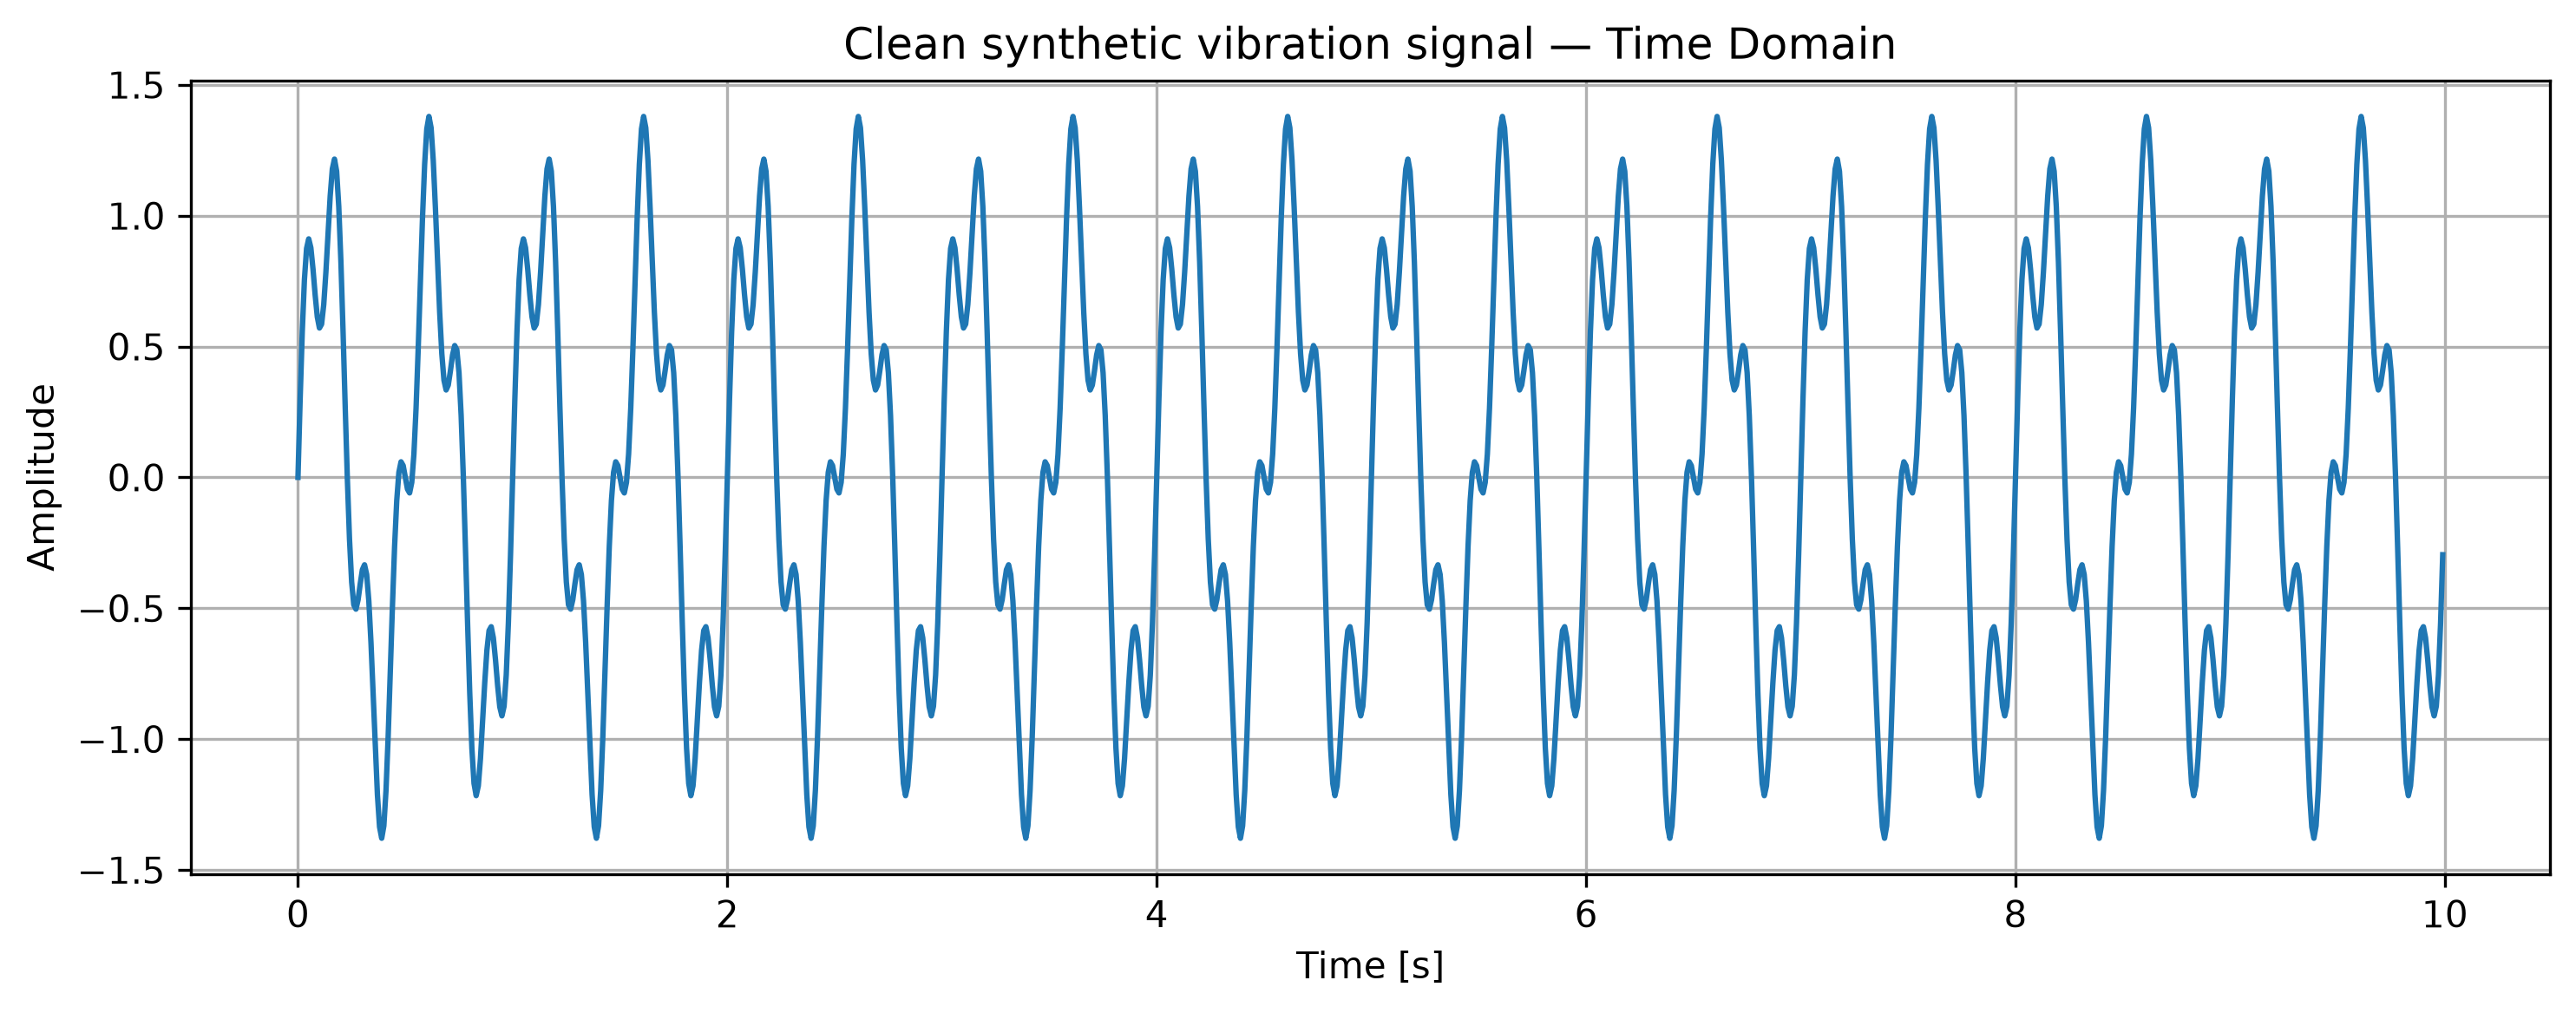
\includegraphics[width=0.92\textwidth]{figures/exp1_time.png}
    \caption{Clean synthetic vibration signal in the time domain.}
\end{figure}

\begin{figure}[H]
    \centering
    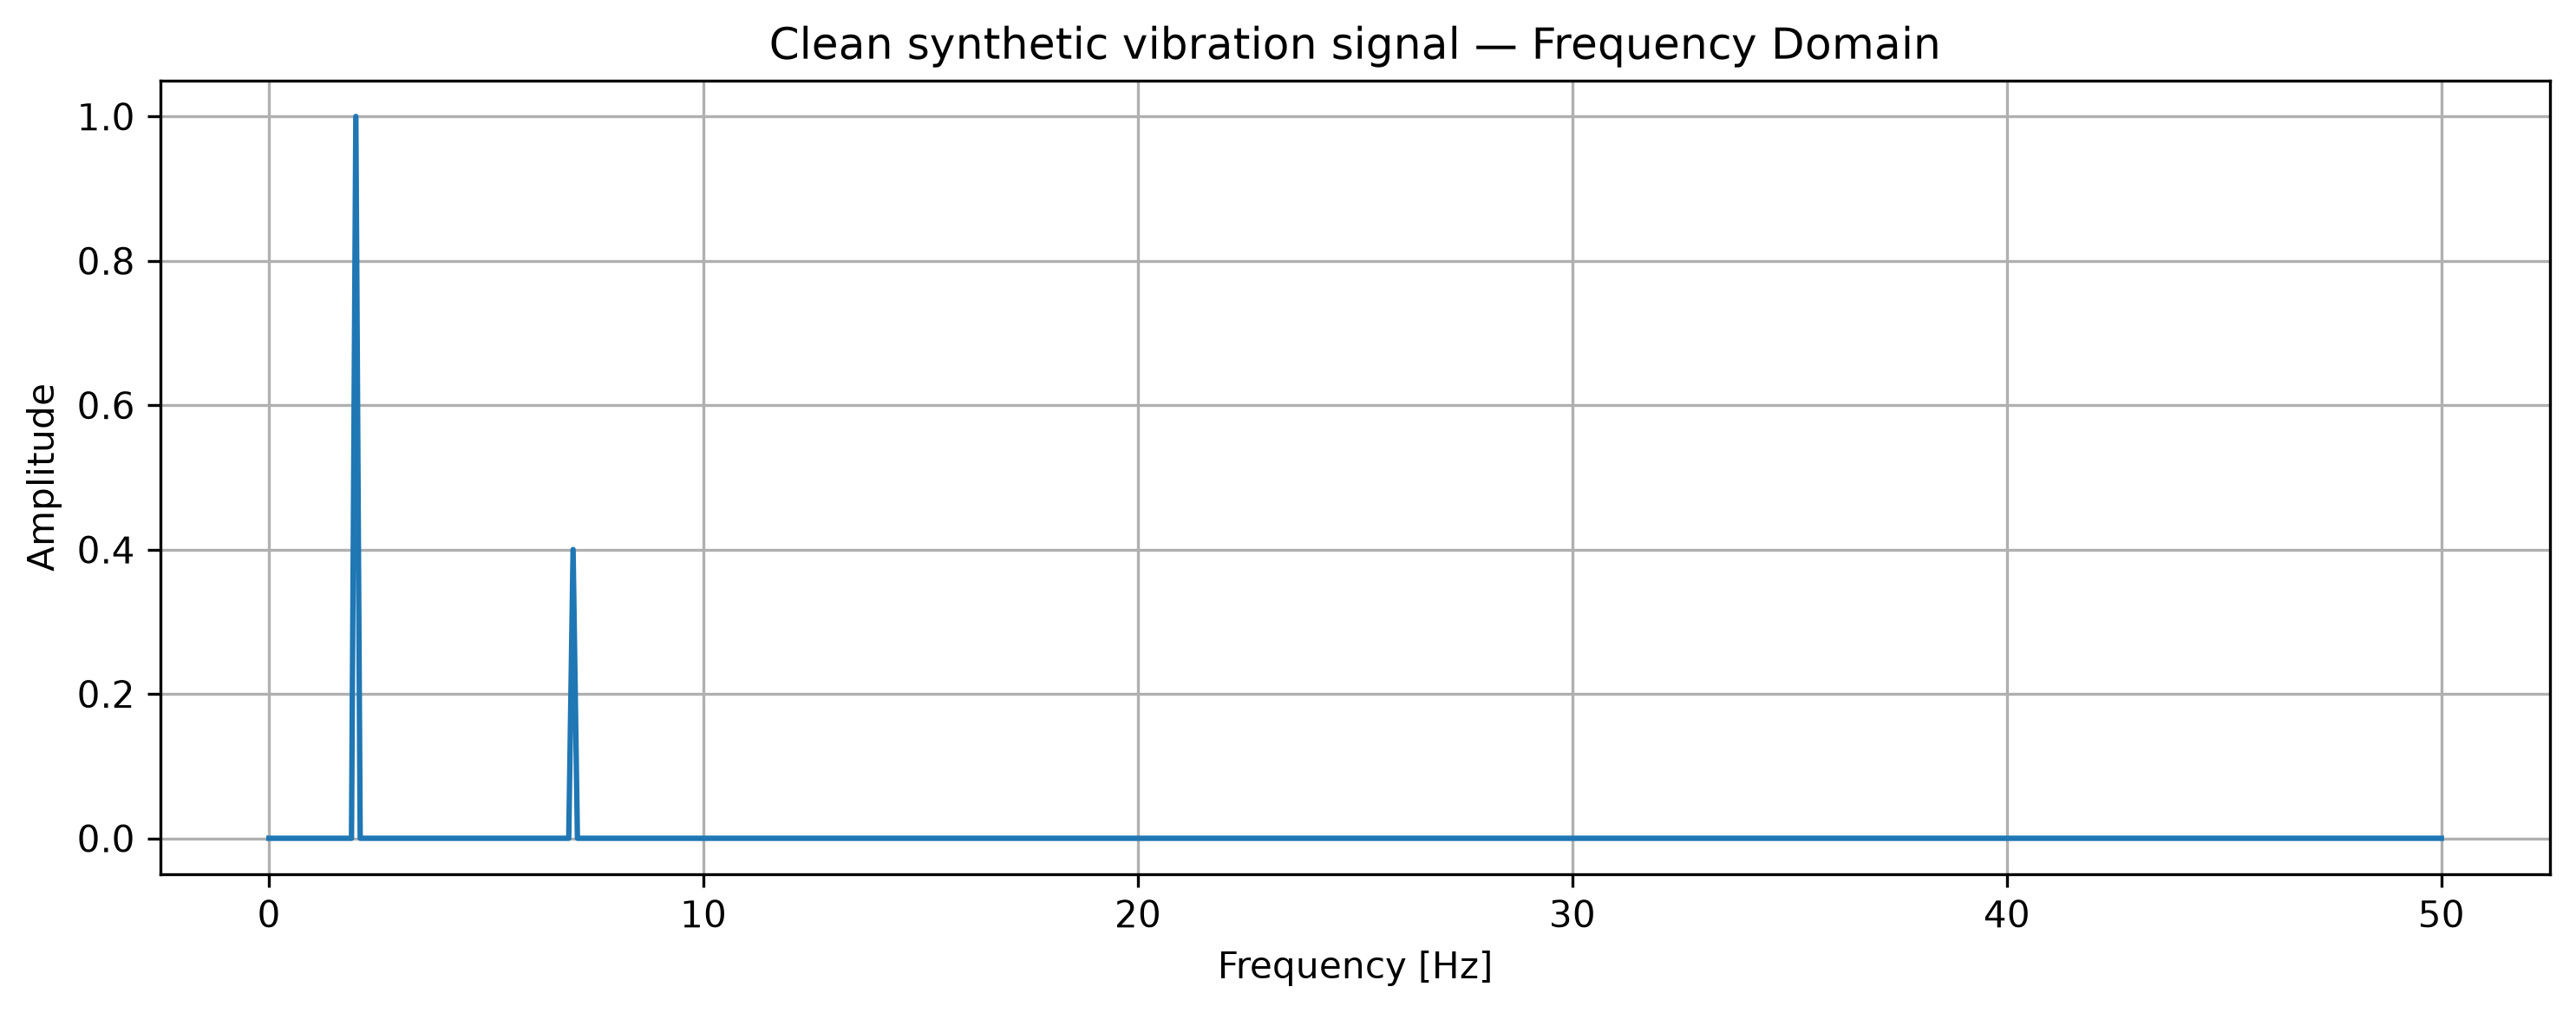
\includegraphics[width=0.92\textwidth]{figures/exp1_frequency.png}
    \caption{FFT amplitude spectrum of the clean signal.}
\end{figure}

\subsection{Observations}

\begin{itemize}
    \item The sampling rate was significantly higher than twice the maximum signal frequency.
    \item The Nyquist frequency was \SI{50}{Hz}, which safely exceeded the highest signal component of \SI{7}{Hz}.
    \item The FFT spectrum showed clear peaks at the known input frequencies.
\end{itemize}

\subsection{Discussion}

This experiment confirms that the signal generation and FFT implementation are functioning correctly. When the sampling condition is satisfied and the signal is noise-free, the frequency-domain representation directly recovers the known sinusoidal components.

% ---------------------------------------------------------
\section{Experiment 2: Aliasing}

\subsection{Premise}

The second experiment investigates aliasing by reducing the sampling frequency while keeping the original signal unchanged.

\begin{table}[H]
\centering
\caption{Experiment 2 parameters.}
\label{tab:exp2_params}
\begin{tabular}{cc}
\toprule
Parameter & Value \\
\midrule
Sampling frequency, \(f_s\) & \SI{10}{Hz} \\
Duration, \(T\) & \SI{10}{s} \\
Nyquist frequency, \(f_N\) & \SI{5}{Hz} \\
Frequency resolution, \(\Delta f\) & \SI{0.1}{Hz} \\
Noise standard deviation, \(\sigma\) & 0.0 \\
\bottomrule
\end{tabular}
\end{table}

The \SI{2}{Hz} component is below the Nyquist frequency and should be preserved. The \SI{7}{Hz} component is above the Nyquist frequency and should be aliased.

The expected aliased frequency is

\begin{equation}
f_{\text{alias}} = |10 - 7| = \SI{3}{Hz}
\end{equation}

\subsection{Results}

The FFT showed peaks at approximately \SI{2}{Hz} and \SI{3}{Hz}. The \SI{3}{Hz} peak is not a true physical component of the original signal. It is the aliased representation of the original \SI{7}{Hz} component.

\begin{figure}[H]
    \centering
    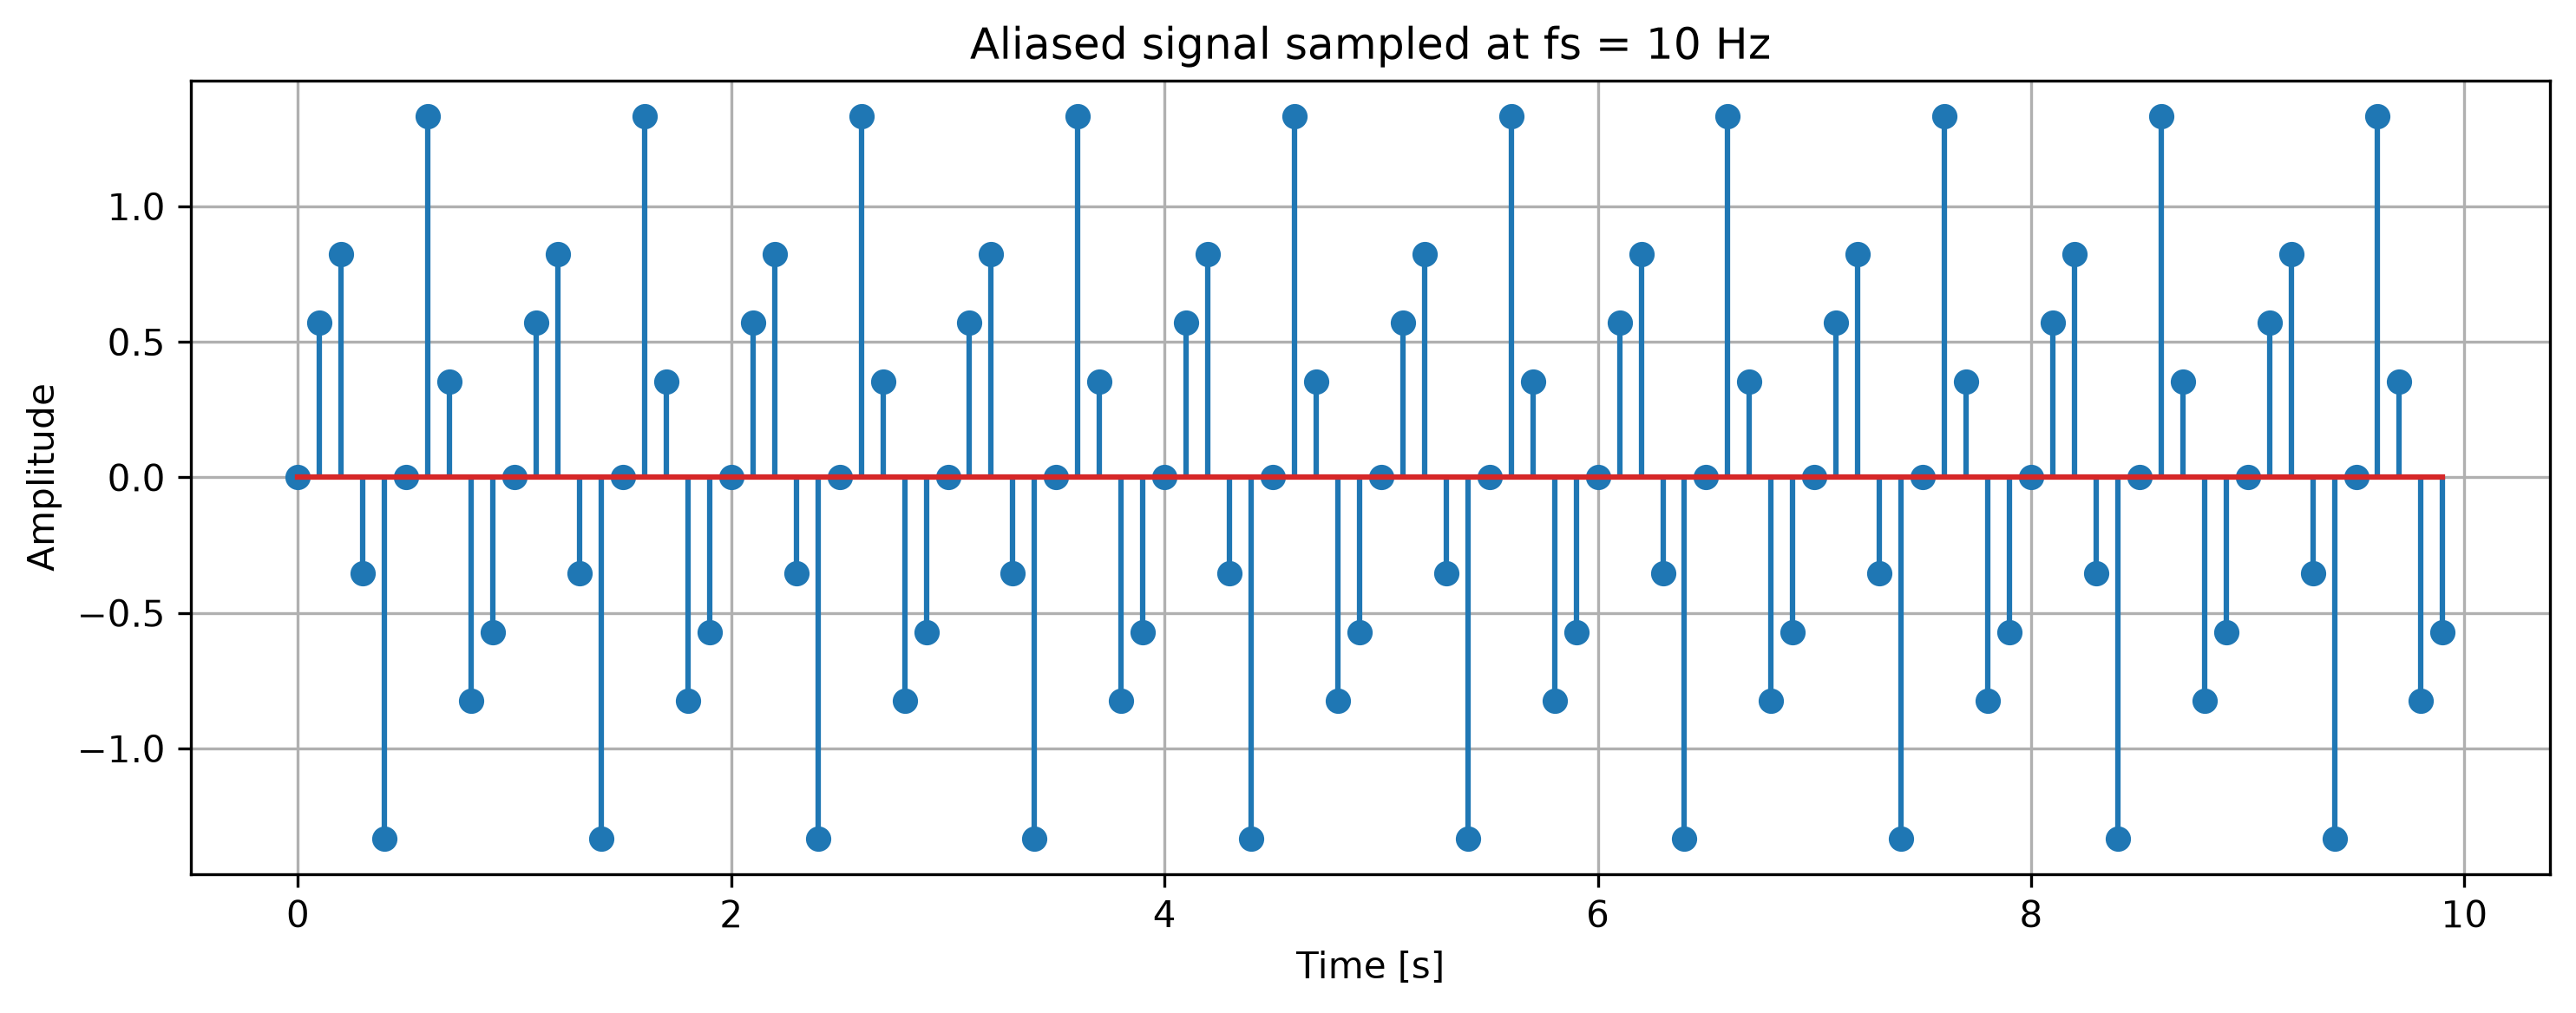
\includegraphics[width=0.92\textwidth]{figures/exp2_stem_time.png}
    \caption{Aliased signal sampled at \SI{10}{Hz}.}
\end{figure}

\begin{figure}[H]
    \centering
    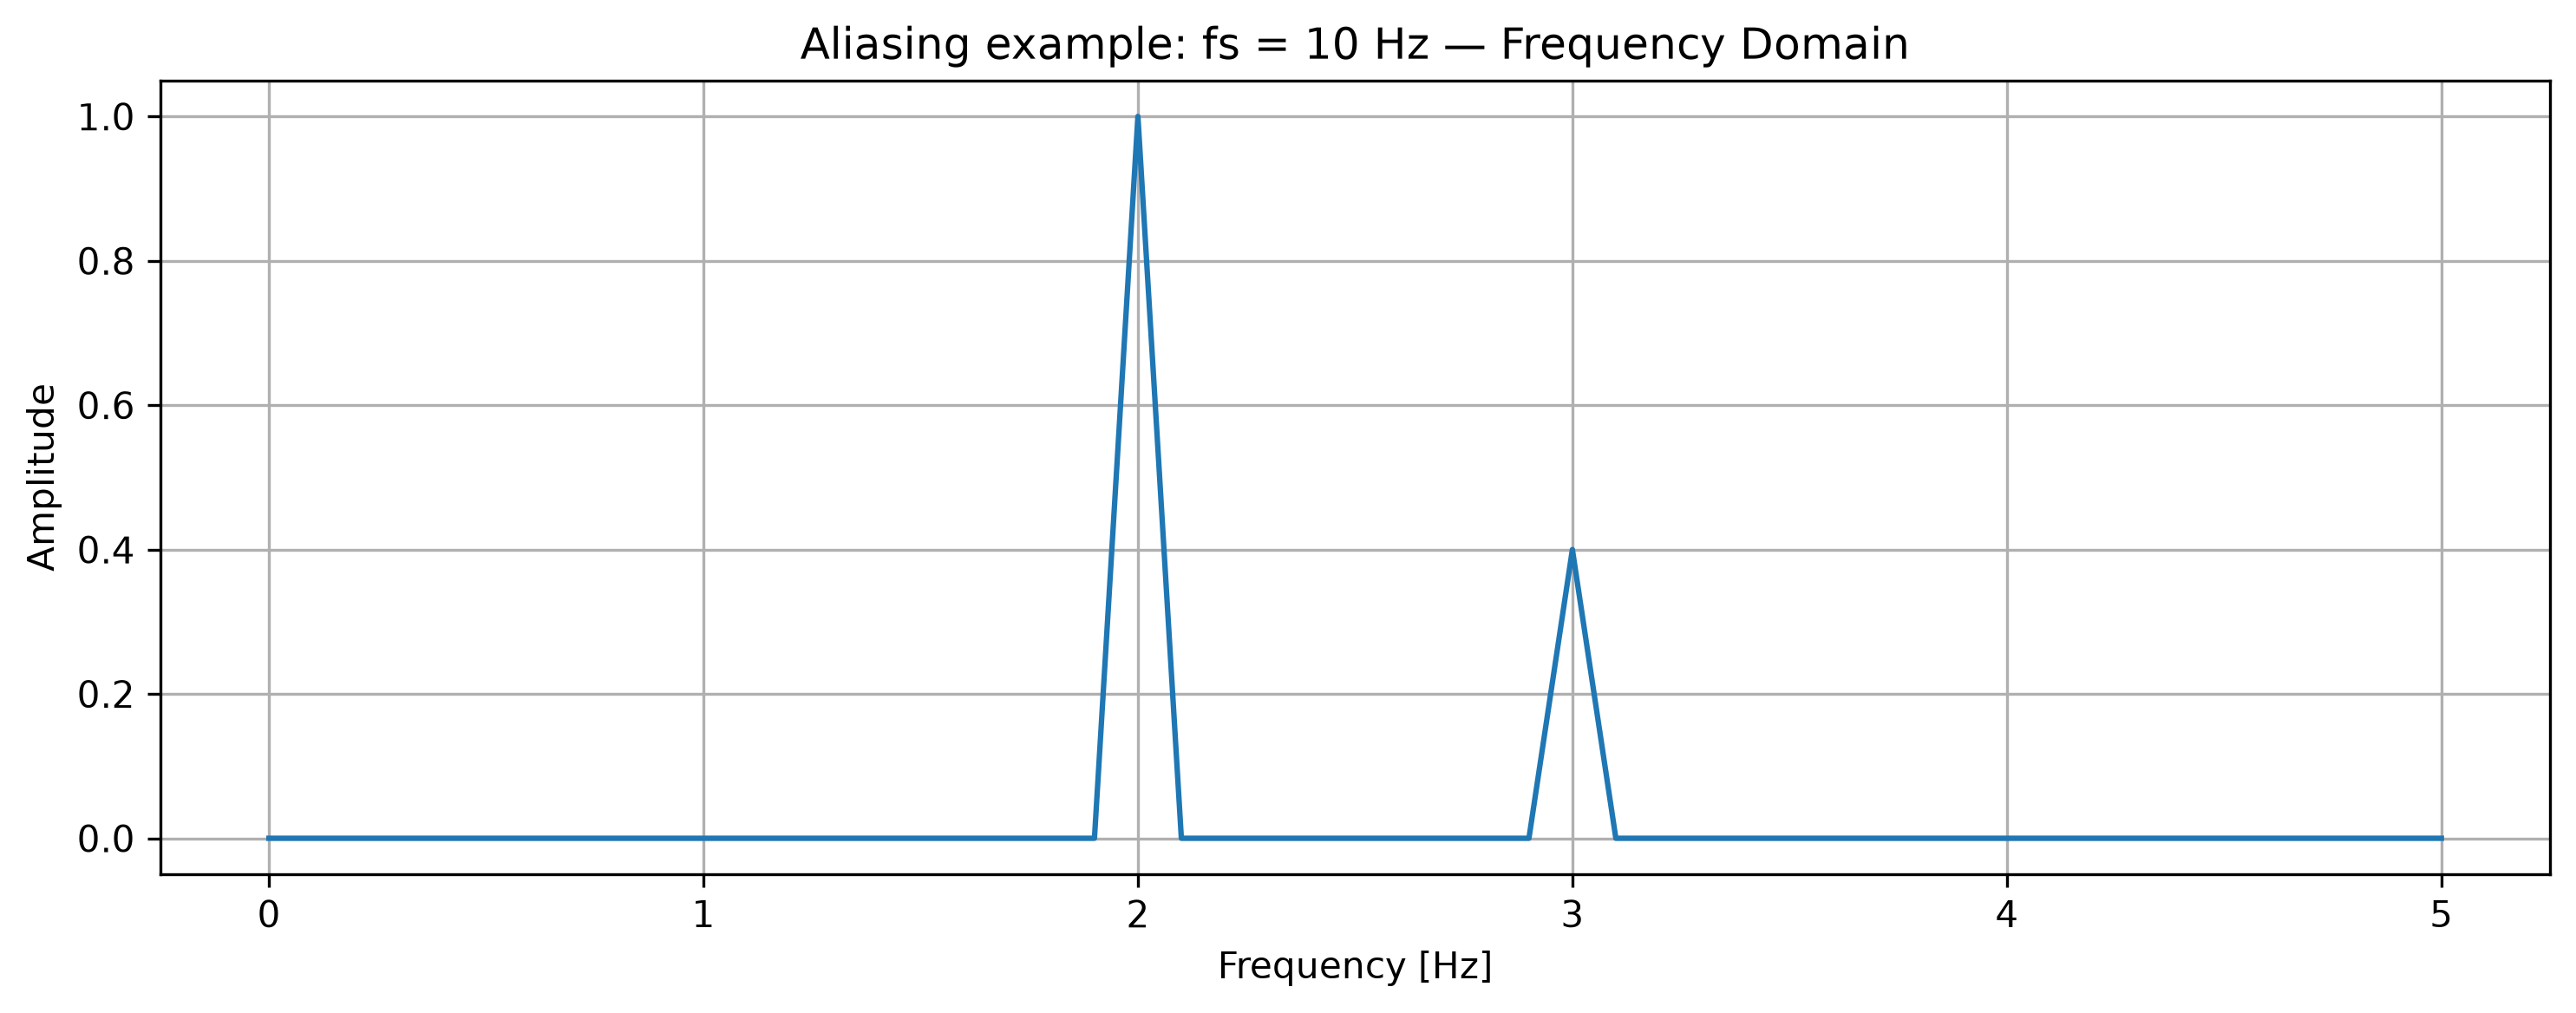
\includegraphics[width=0.92\textwidth]{figures/exp2_frequency.png}
    \caption{FFT amplitude spectrum showing the aliased \SI{3}{Hz} peak.}
\end{figure}

\subsection{Observations}

\begin{itemize}
    \item The \SI{2}{Hz} component was correctly retained.
    \item The \SI{7}{Hz} component was not correctly represented.
    \item A false peak appeared at approximately \SI{3}{Hz}.
    \item The frequency-domain plot appeared clean, but its physical interpretation was incorrect.
\end{itemize}

\subsection{Discussion}

This experiment demonstrates that the FFT only analyzes the sampled data. It does not know the original continuous-time signal. If the sampling frequency is too low, the frequency spectrum may contain false low-frequency peaks.

For vibration-based SHM, this is critical. A falsely aliased frequency may be mistaken for a structural mode.

% ---------------------------------------------------------
\section{Experiment 3: Noise Sensitivity}

\subsection{Premise}

The third experiment studies the effect of additive Gaussian noise on the time-domain signal and FFT spectrum.

The signal is written as

\begin{equation}
x_{\text{noisy}}(t) = x_{\text{clean}}(t) + \eta(t)
\end{equation}

where

\begin{equation}
\eta(t) \sim \mathcal{N}(0,\sigma^2)
\end{equation}

\begin{table}[H]
\centering
\caption{Experiment 3 parameters.}
\label{tab:exp3_params}
\begin{tabular}{cc}
\toprule
Parameter & Value \\
\midrule
Sampling frequency, \(f_s\) & \SI{100}{Hz} \\
Duration, \(T\) & \SI{10}{s} \\
Nyquist frequency, \(f_N\) & \SI{50}{Hz} \\
Frequency resolution, \(\Delta f\) & \SI{0.1}{Hz} \\
Noise levels, \(\sigma\) & 0.0, 0.2, 0.5, 1.0 \\
\bottomrule
\end{tabular}
\end{table}

\subsection{Results}

As the noise level increased, the time-domain signal became less visually interpretable. The dominant \SI{2}{Hz} peak remained visible for all tested noise levels. The weaker \SI{7}{Hz} peak became harder to identify at higher noise levels.

\begin{table}[H]
\centering
\caption{Experiment 3 result summary.}
\label{tab:exp3_results}
\begin{tabular}{cccc}
\toprule
Noise Std., \(\sigma\) & SNR [dB] & Dominant Peak & Secondary Peak \\
\midrule
0.0 & \(\infty\) & \SI{2}{Hz} & \SI{7}{Hz} \\
0.2 & 11.72 & \SI{2}{Hz} & \SI{7}{Hz} \\
0.5 & 3.76 & \SI{2}{Hz} & \SI{7}{Hz} or reduced clarity \\
1.0 & -2.26 & \SI{2}{Hz} & weak or partially masked \\
\bottomrule
\end{tabular}
\end{table}

\begin{figure}[H]
    \centering
    \begin{subfigure}{0.48\textwidth}
        \centering
        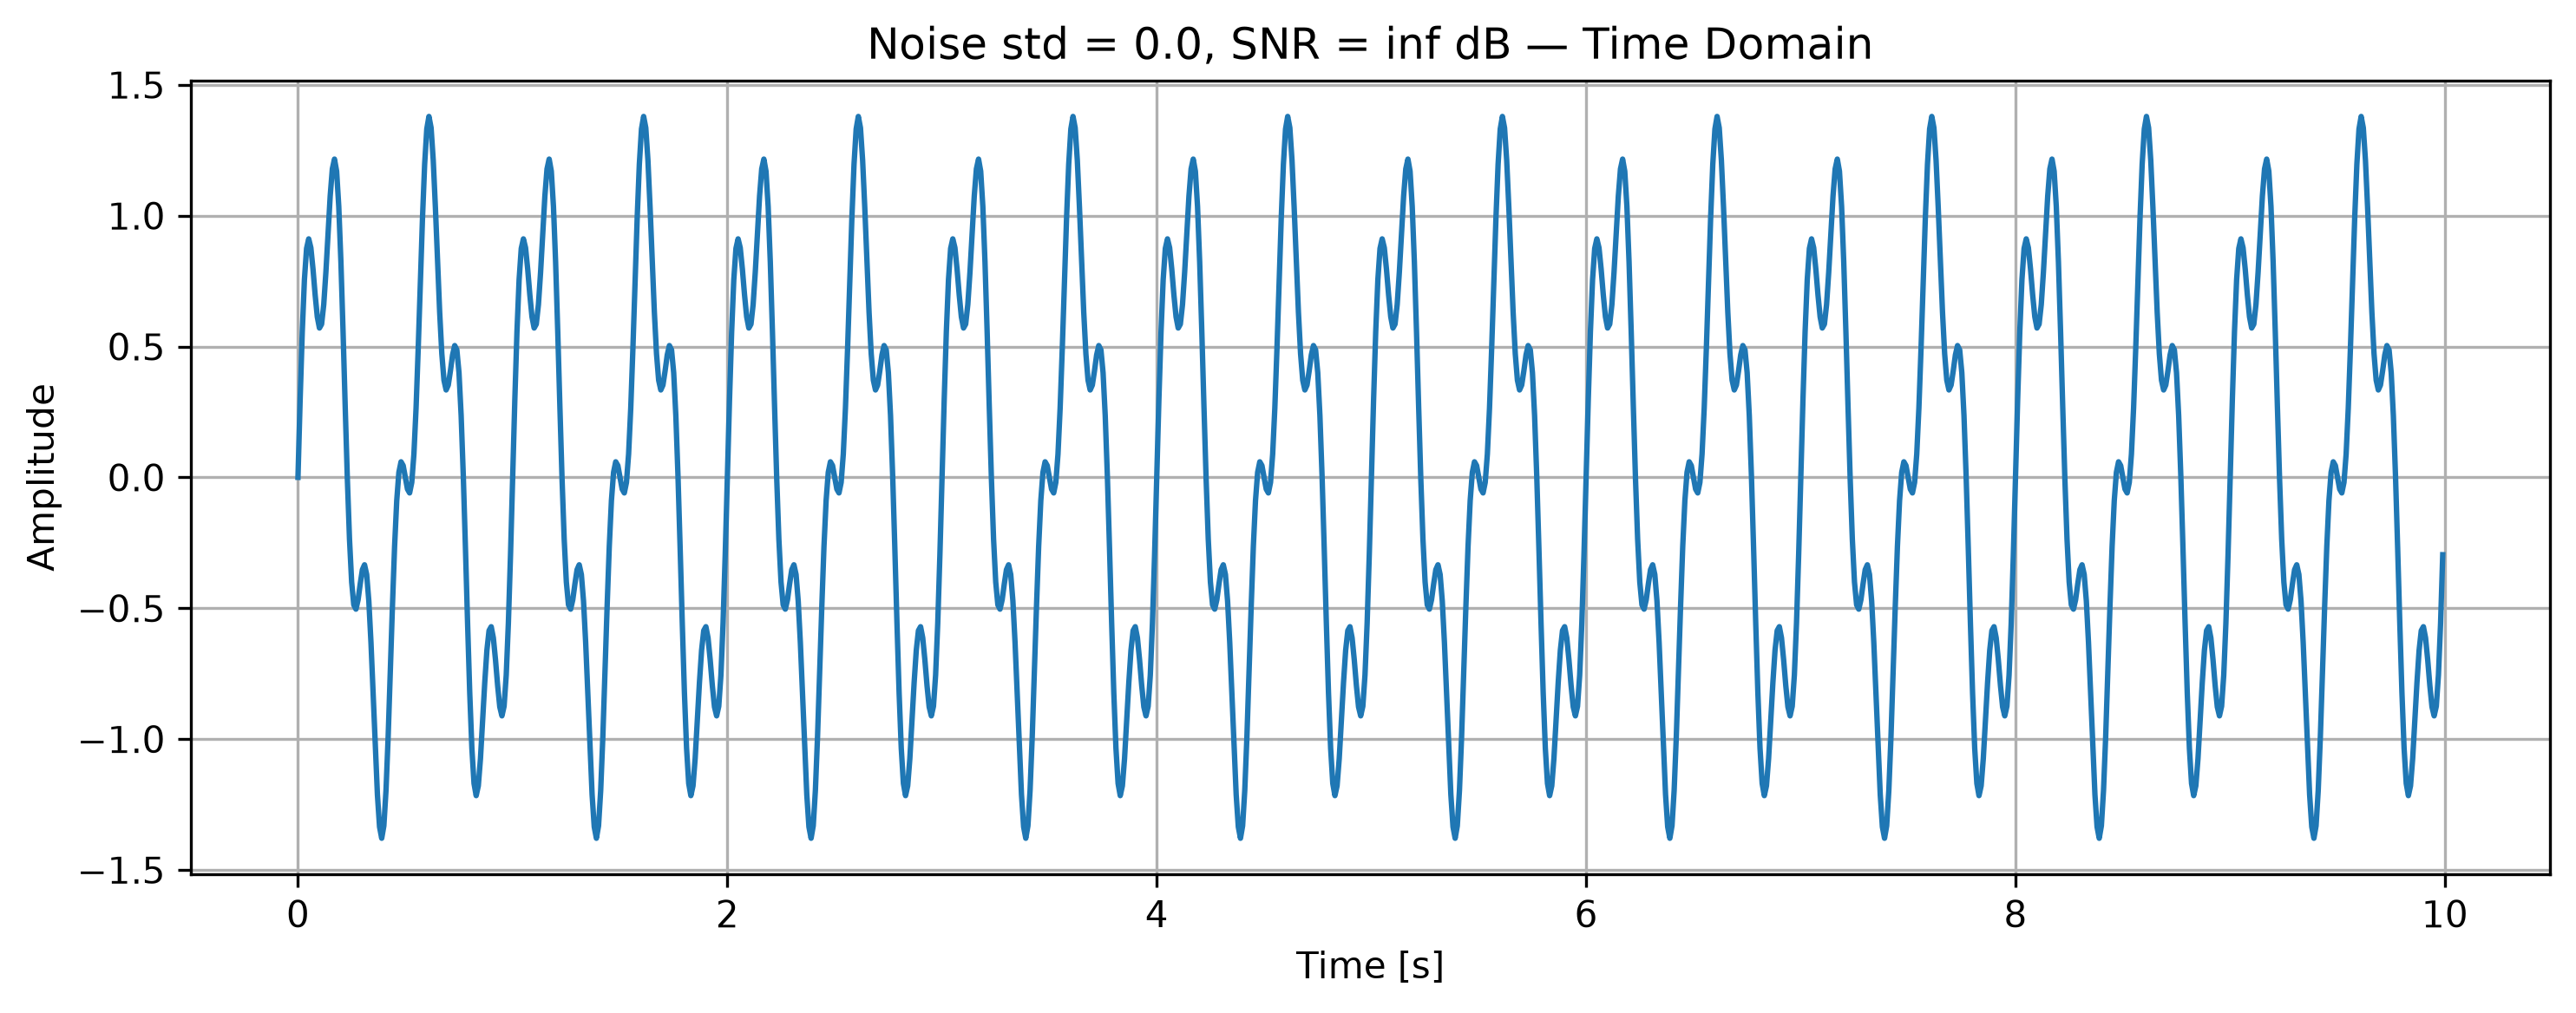
\includegraphics[width=\textwidth]{figures/exp3_sigma_0_0_time.png}
        \caption{Time domain.}
    \end{subfigure}
    \hfill
    \begin{subfigure}{0.48\textwidth}
        \centering
        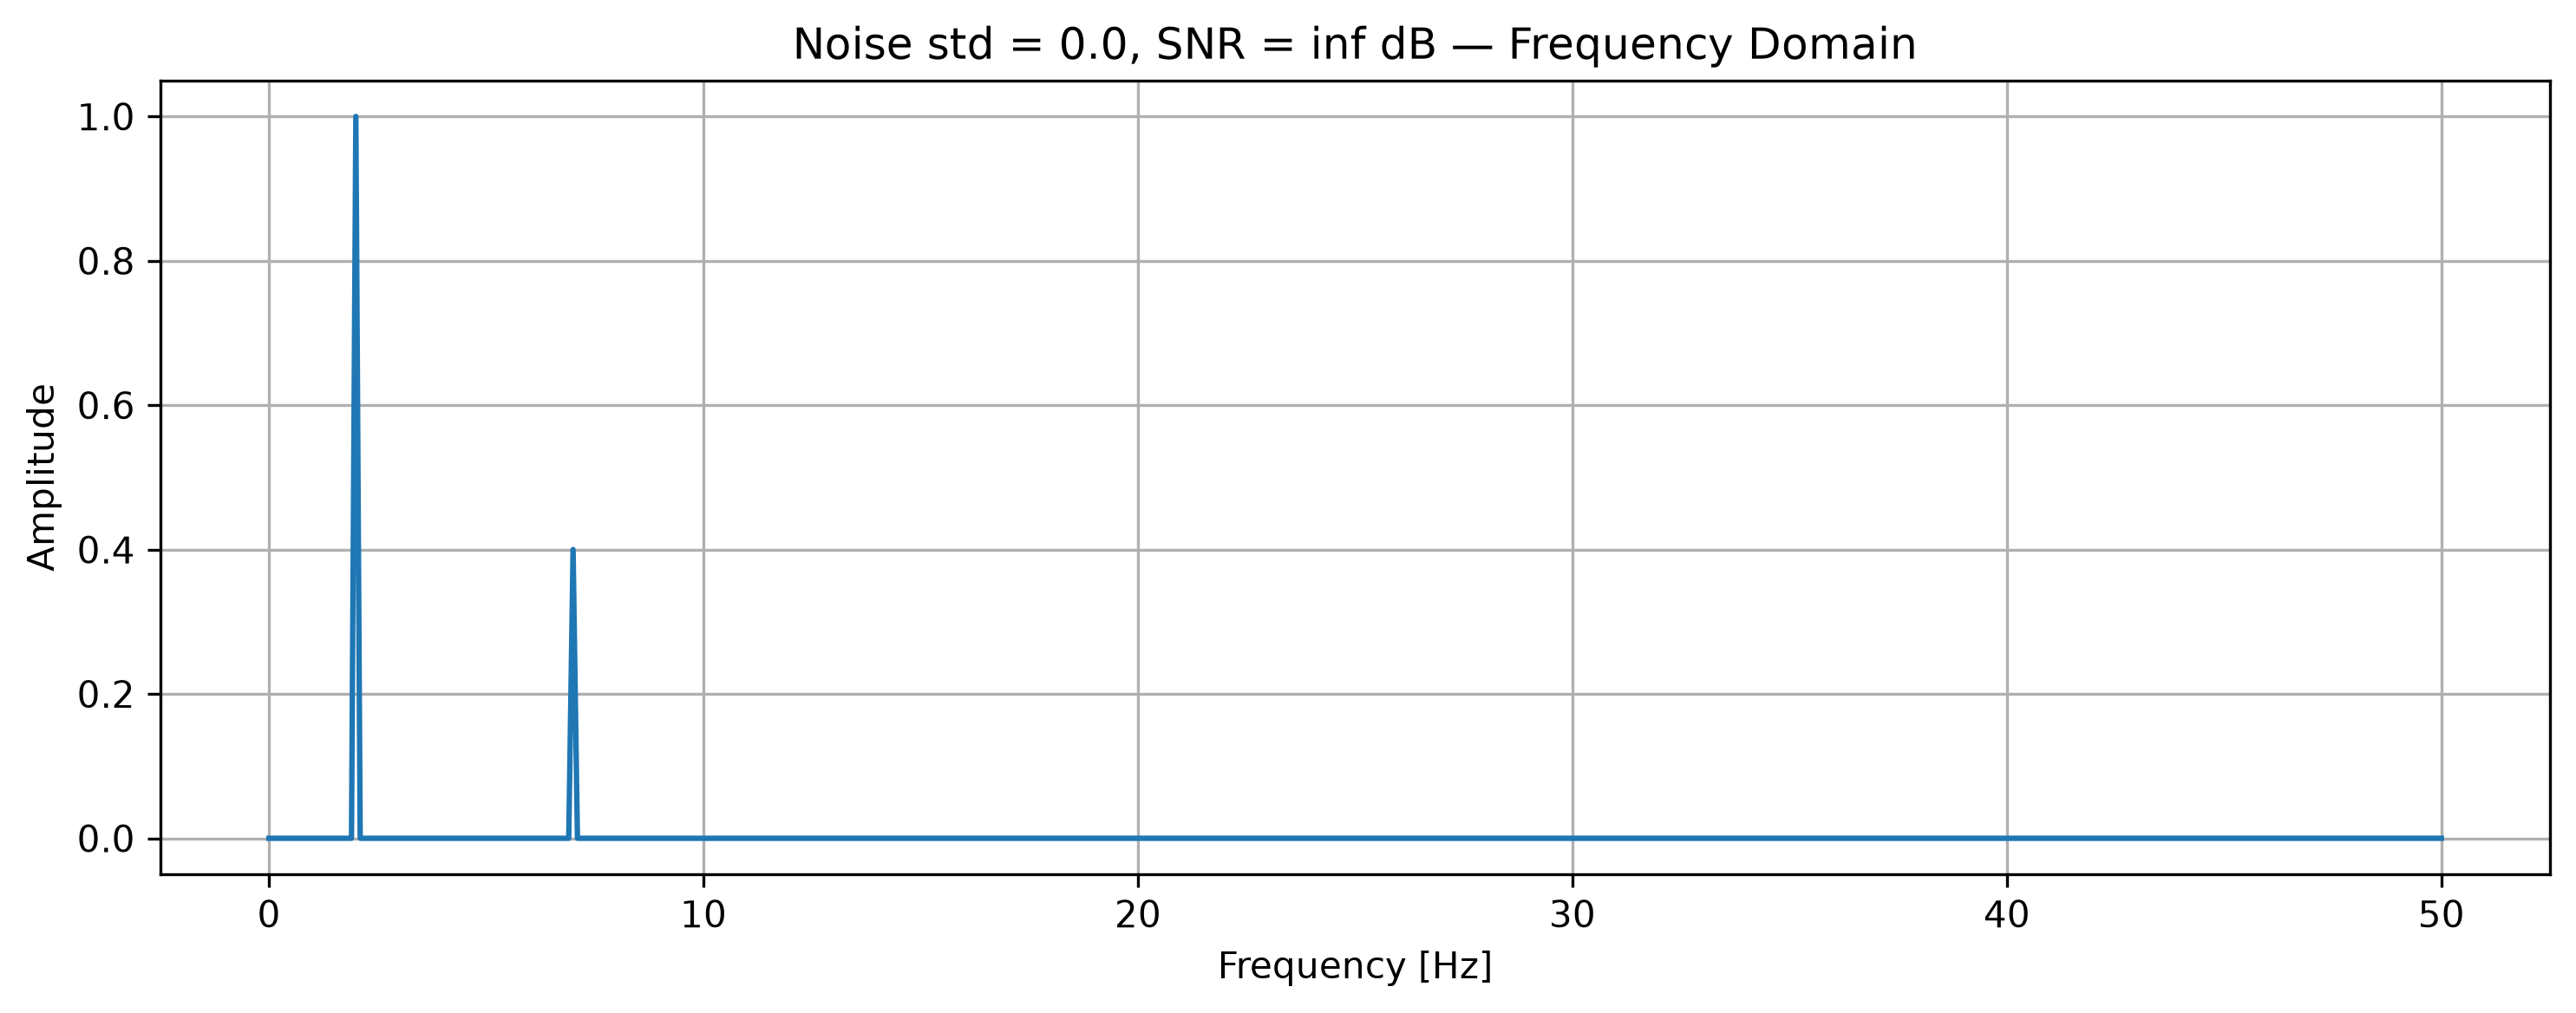
\includegraphics[width=\textwidth]{figures/exp3_sigma_0_0_frequency.png}
        \caption{Frequency domain.}
    \end{subfigure}
    \caption{Noise sensitivity result for \(\sigma = 0.0\).}
\end{figure}

\begin{figure}[H]
    \centering
    \begin{subfigure}{0.48\textwidth}
        \centering
        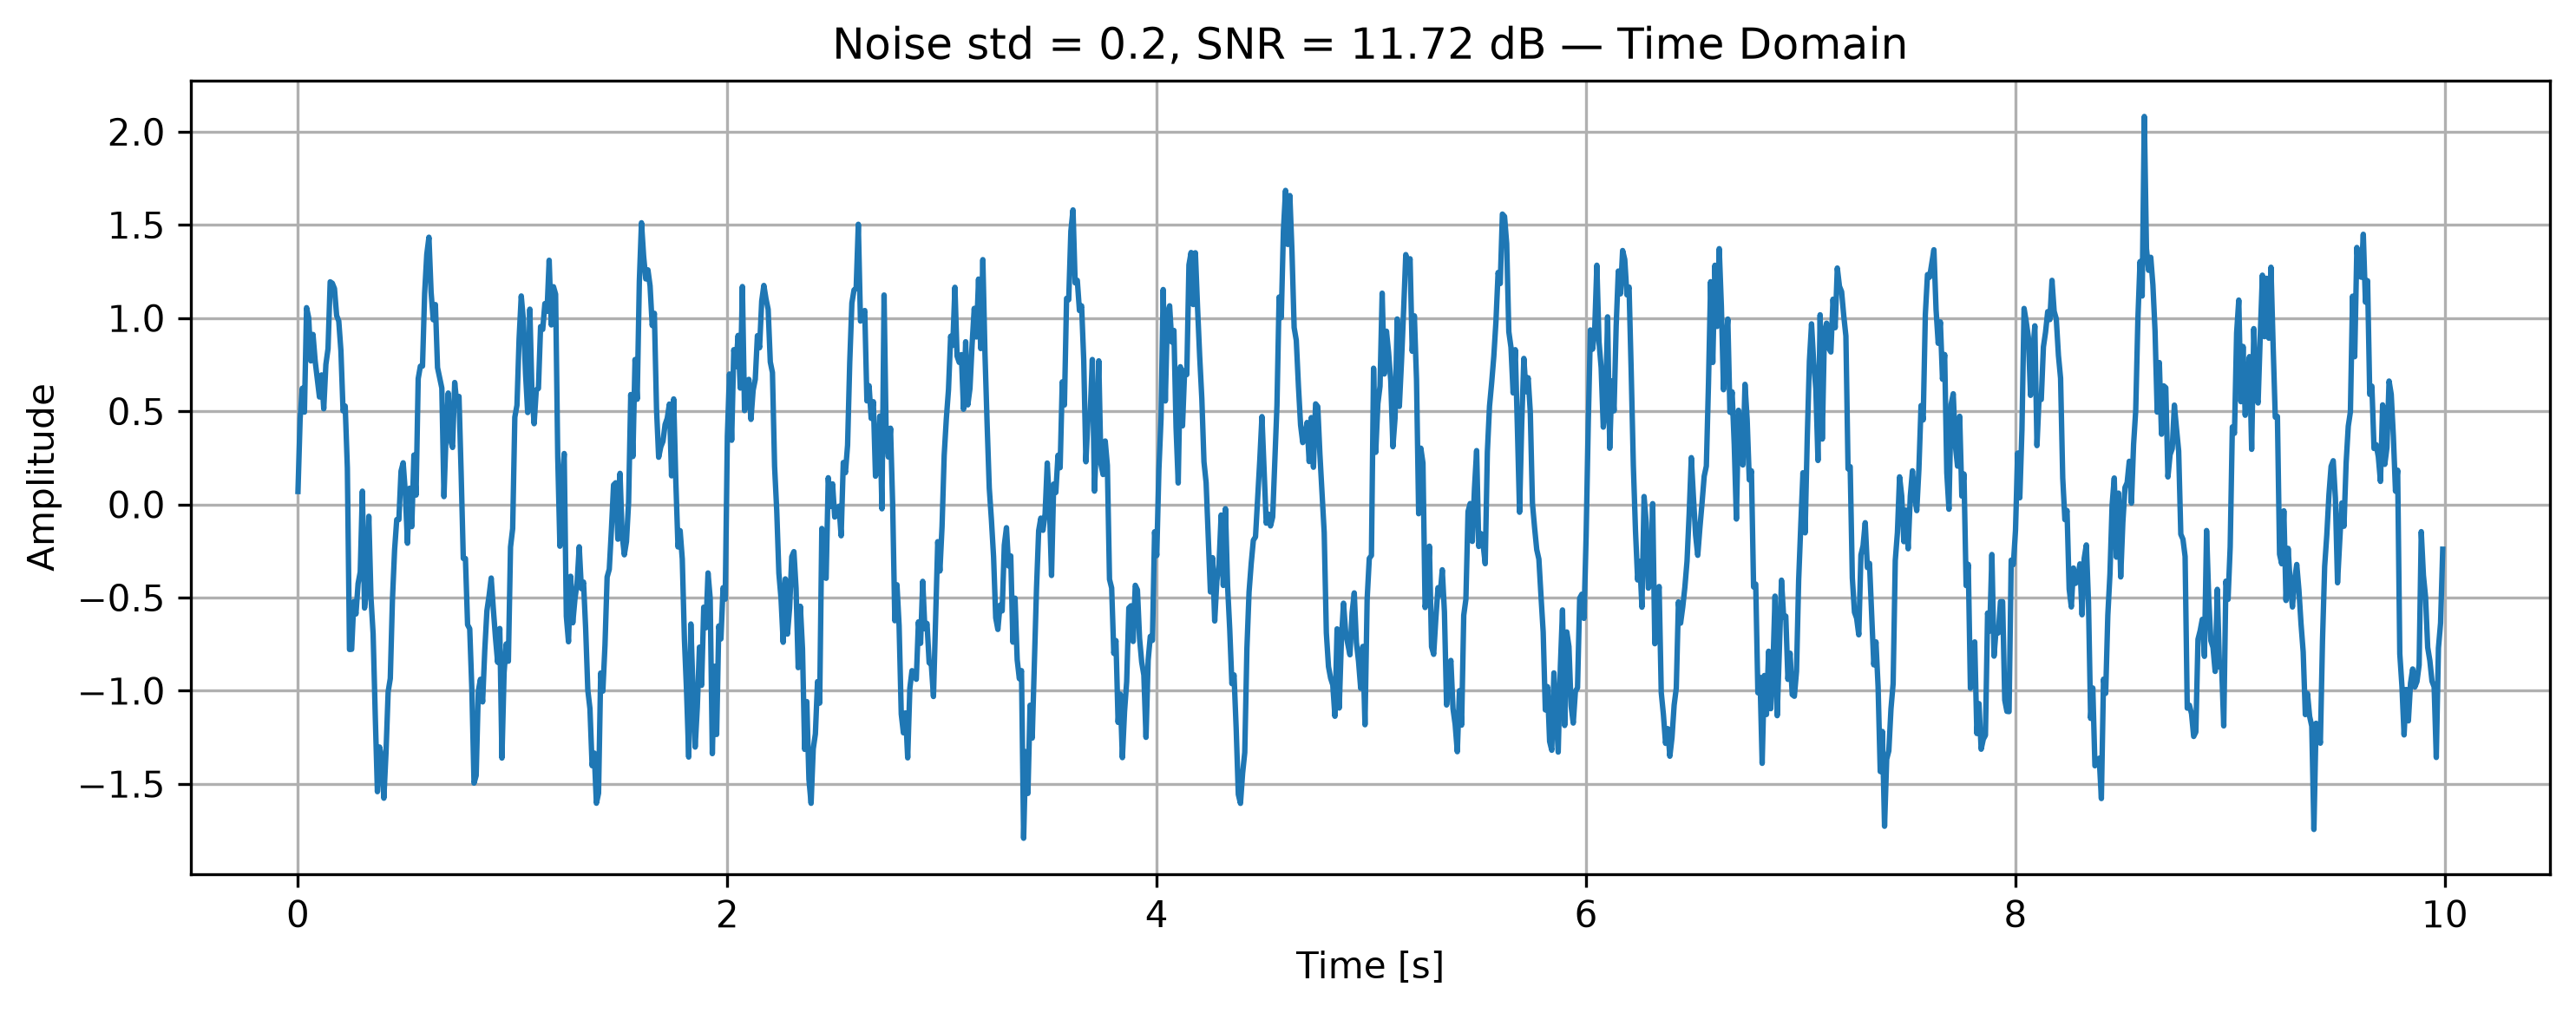
\includegraphics[width=\textwidth]{figures/exp3_sigma_0_2_time.png}
        \caption{Time domain.}
    \end{subfigure}
    \hfill
    \begin{subfigure}{0.48\textwidth}
        \centering
        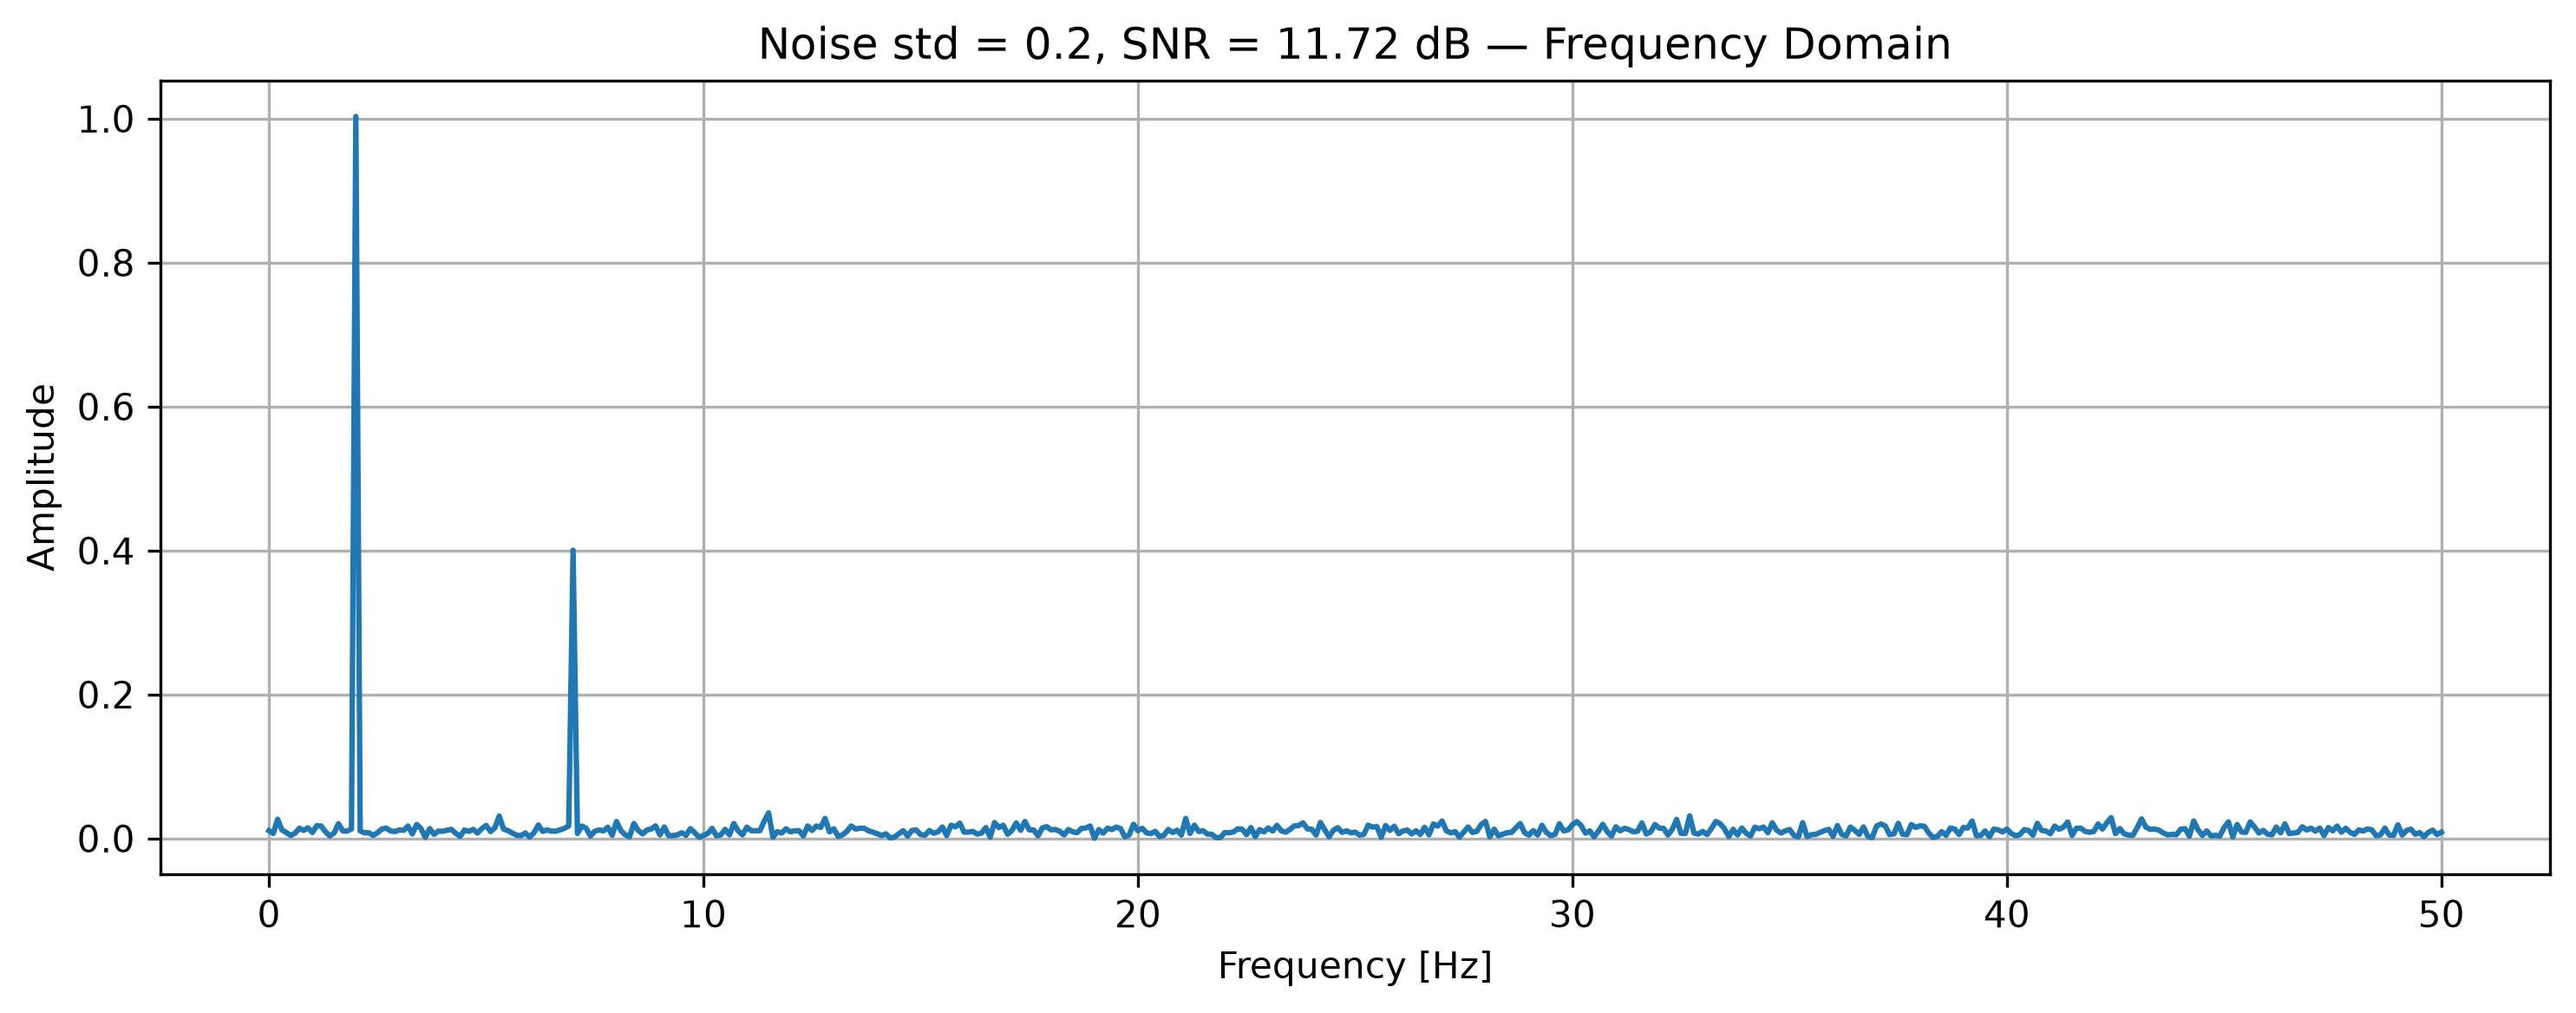
\includegraphics[width=\textwidth]{figures/exp3_sigma_0_2_frequency.png}
        \caption{Frequency domain.}
    \end{subfigure}
    \caption{Noise sensitivity result for \(\sigma = 0.2\).}
\end{figure}

\begin{figure}[H]
    \centering
    \begin{subfigure}{0.48\textwidth}
        \centering
        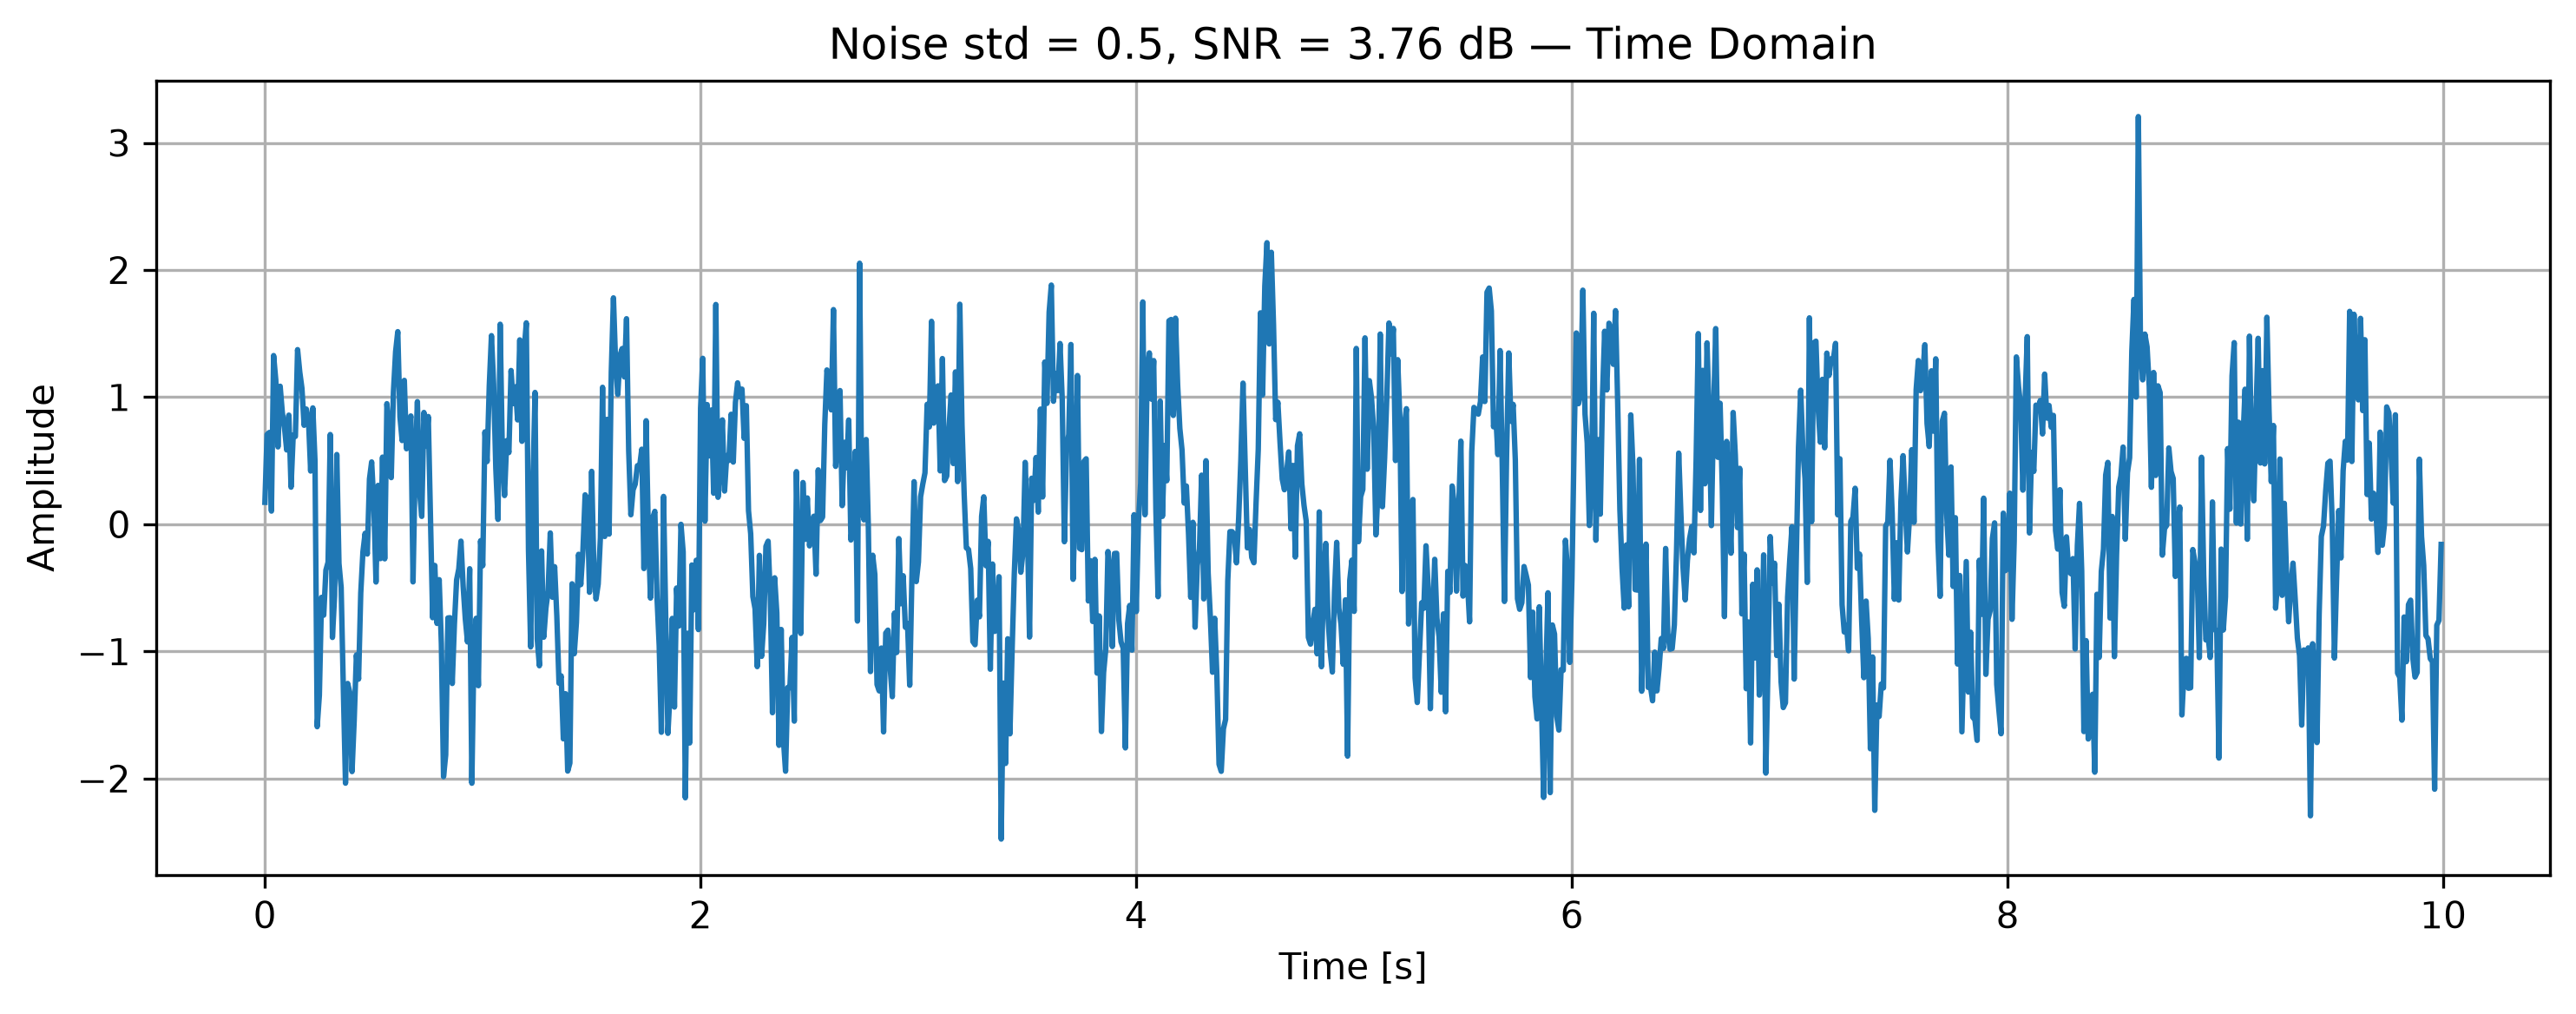
\includegraphics[width=\textwidth]{figures/exp3_sigma_0_5_time.png}
        \caption{Time domain.}
    \end{subfigure}
    \hfill
    \begin{subfigure}{0.48\textwidth}
        \centering
        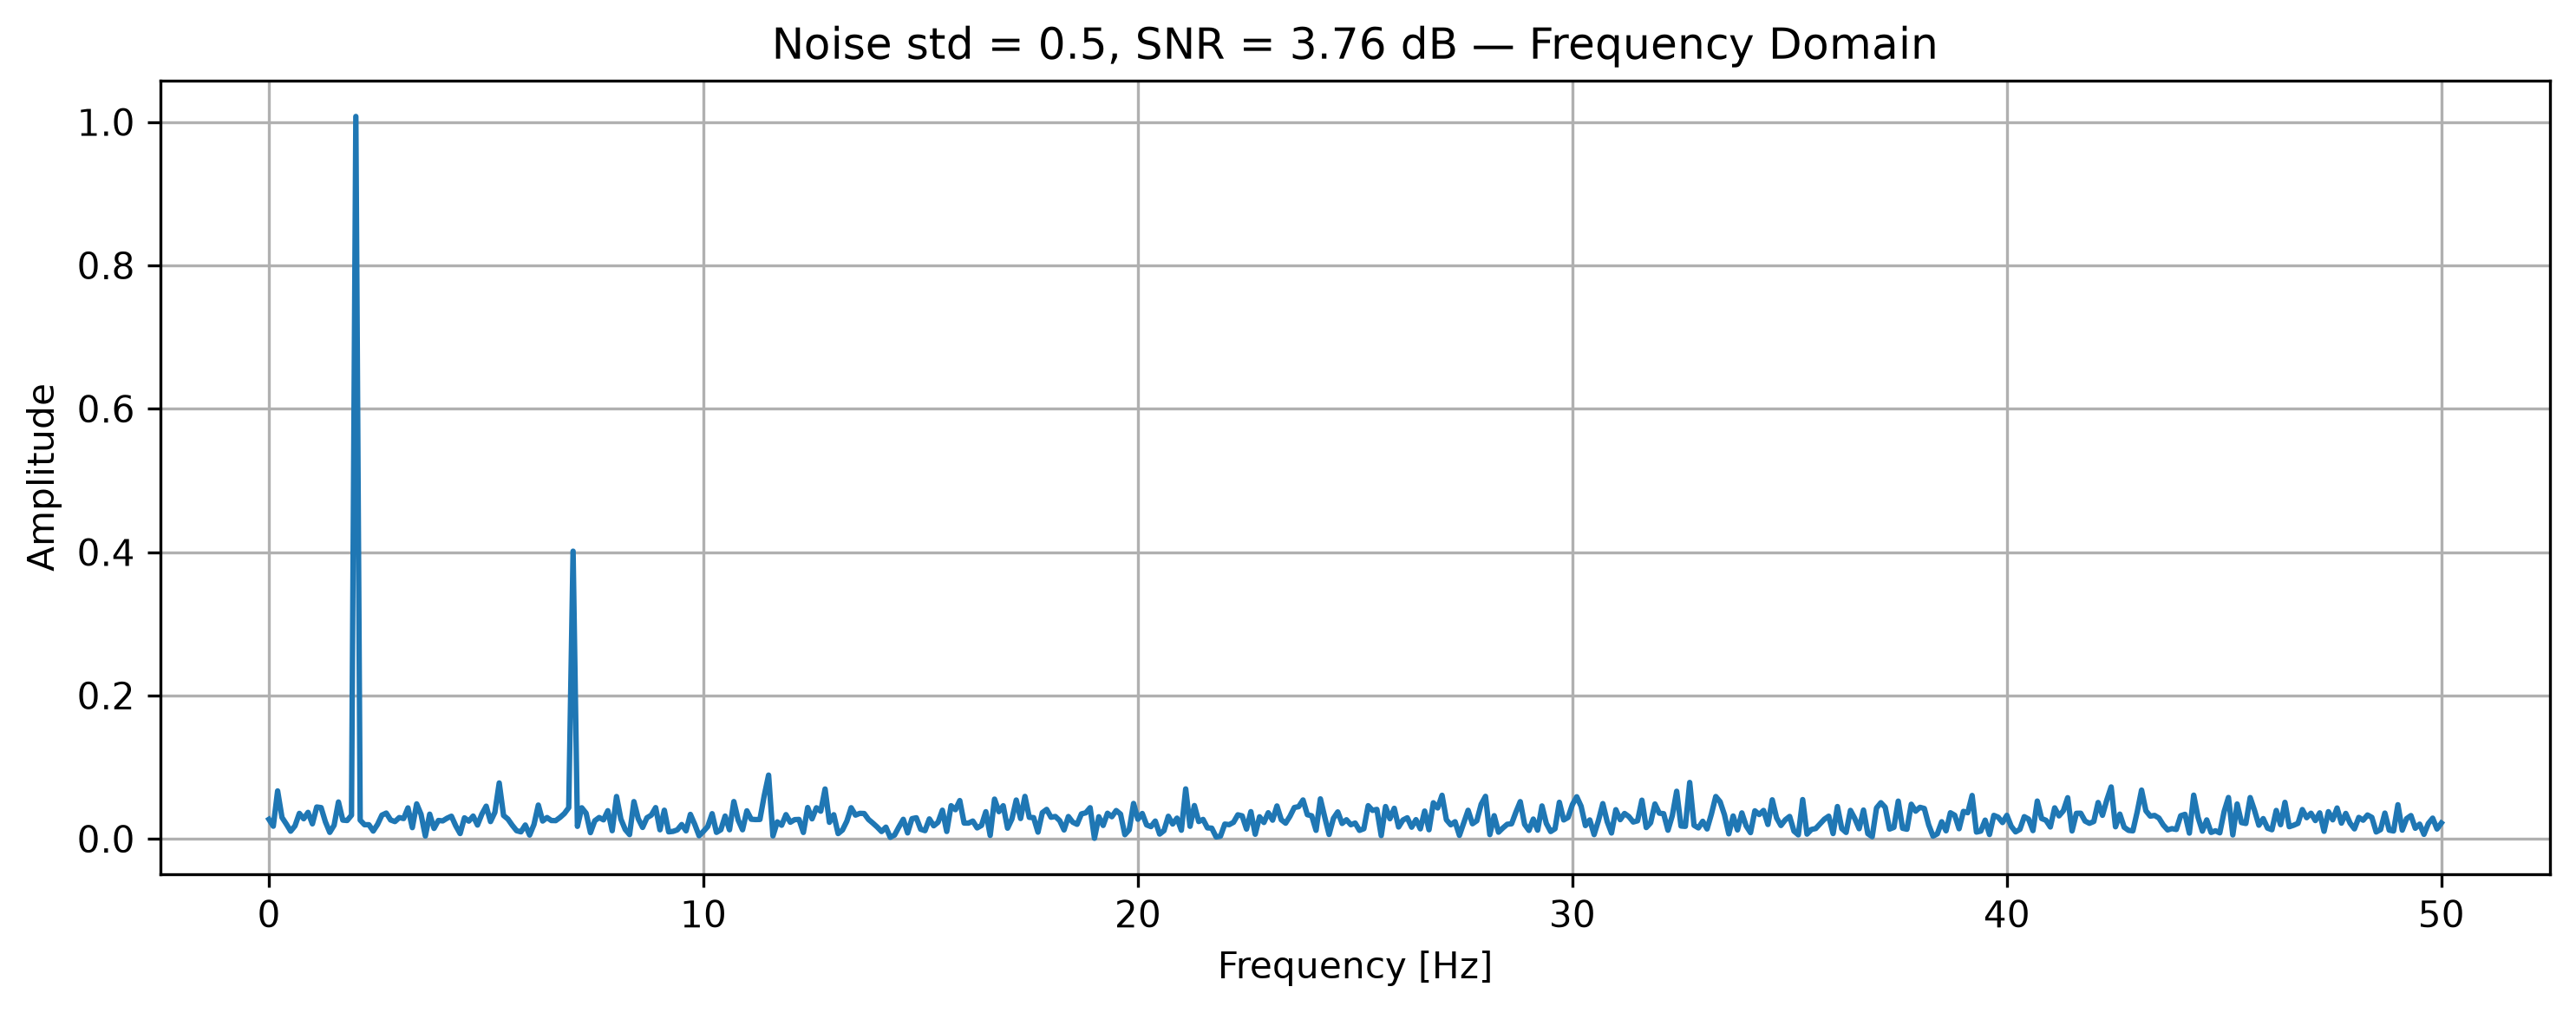
\includegraphics[width=\textwidth]{figures/exp3_sigma_0_5_frequency.png}
        \caption{Frequency domain.}
    \end{subfigure}
    \caption{Noise sensitivity result for \(\sigma = 0.5\).}
\end{figure}

\begin{figure}[H]
    \centering
    \begin{subfigure}{0.48\textwidth}
        \centering
        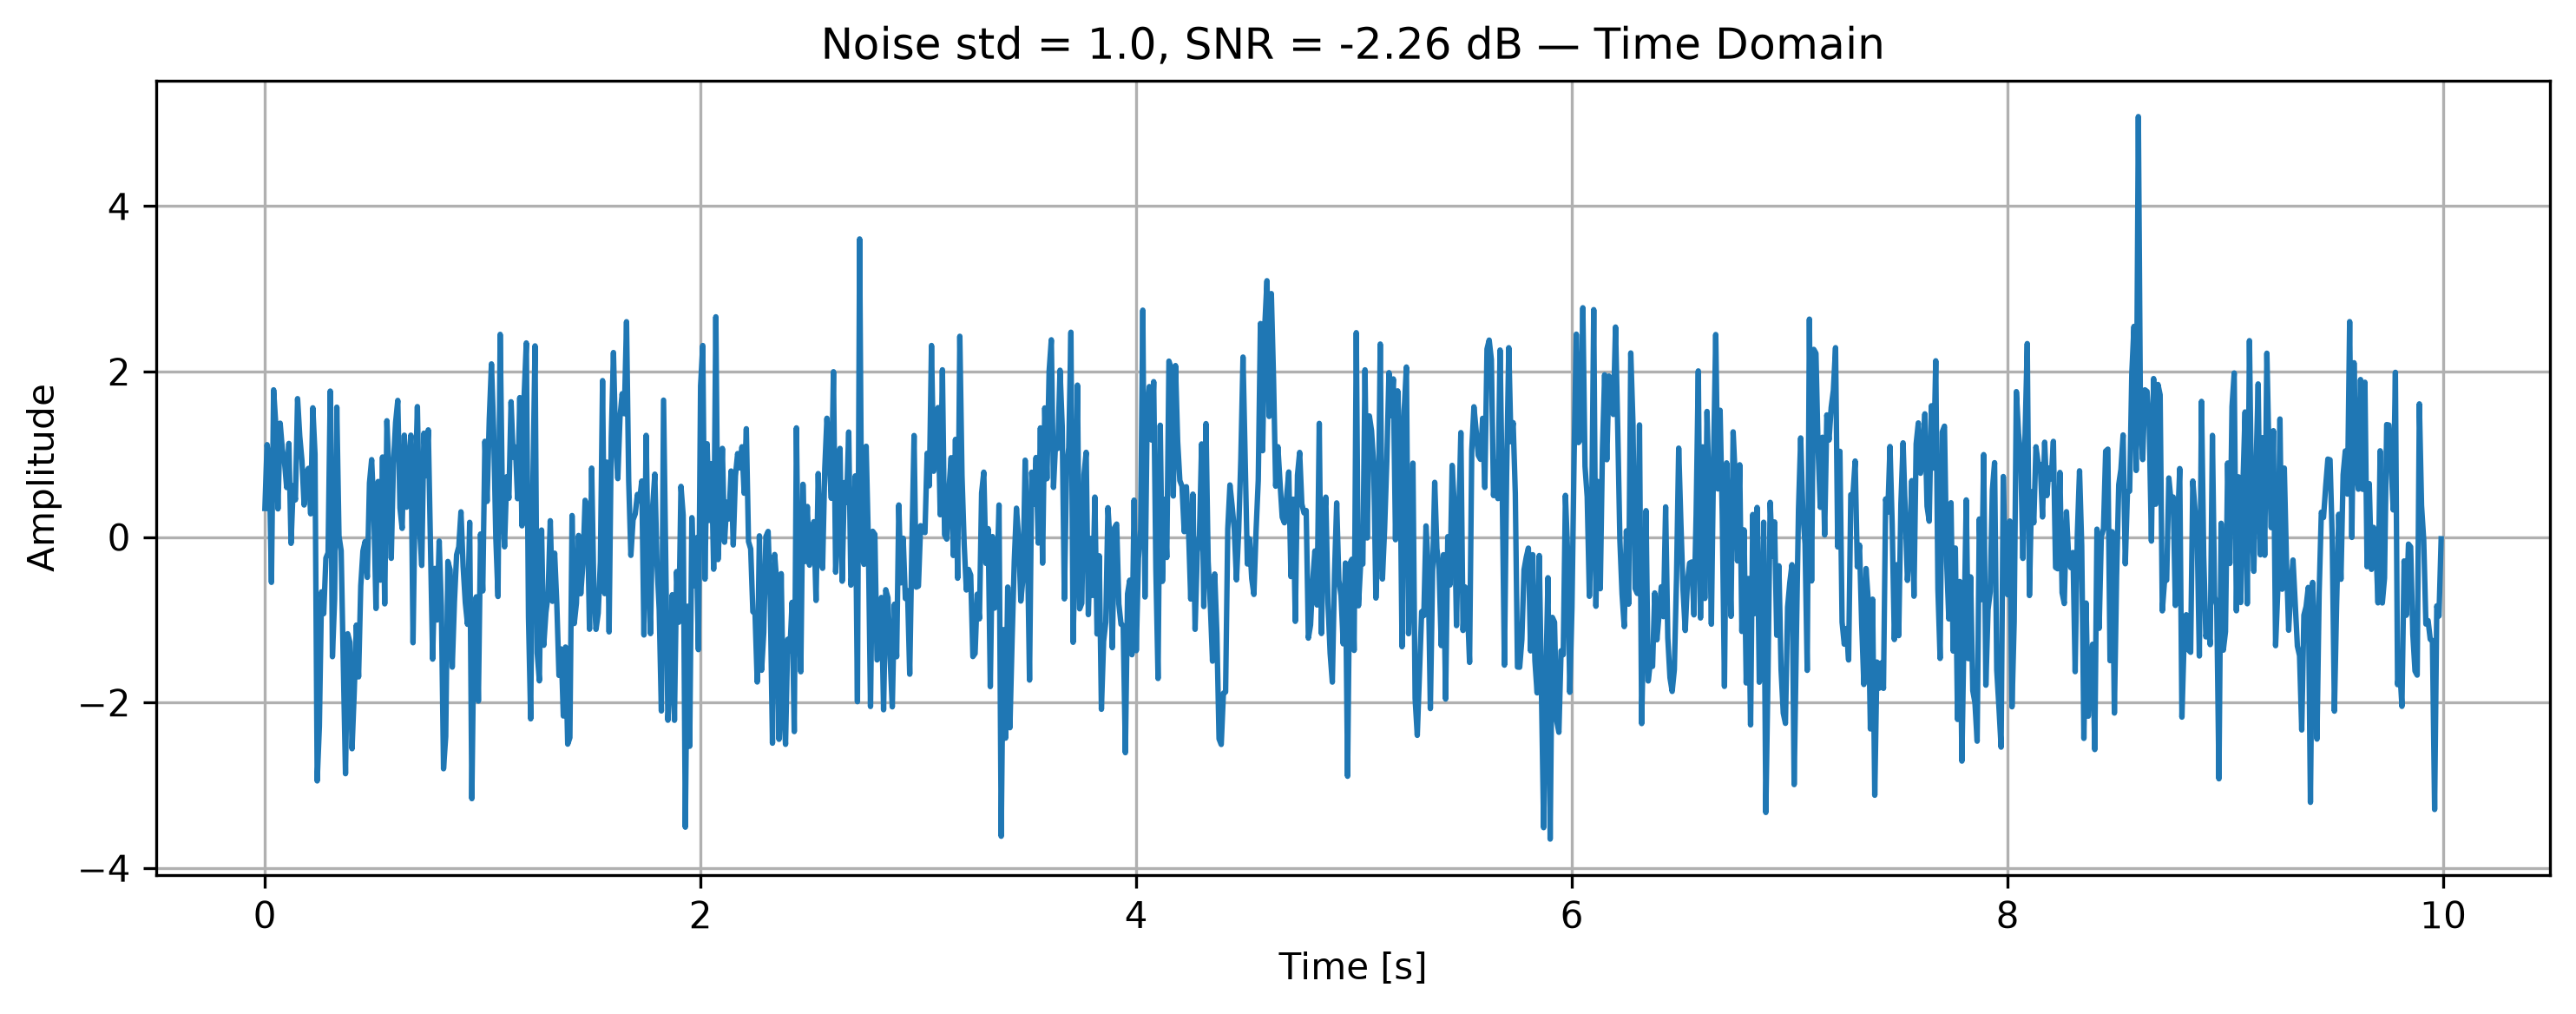
\includegraphics[width=\textwidth]{figures/exp3_sigma_1_0_time.png}
        \caption{Time domain.}
    \end{subfigure}
    \hfill
    \begin{subfigure}{0.48\textwidth}
        \centering
        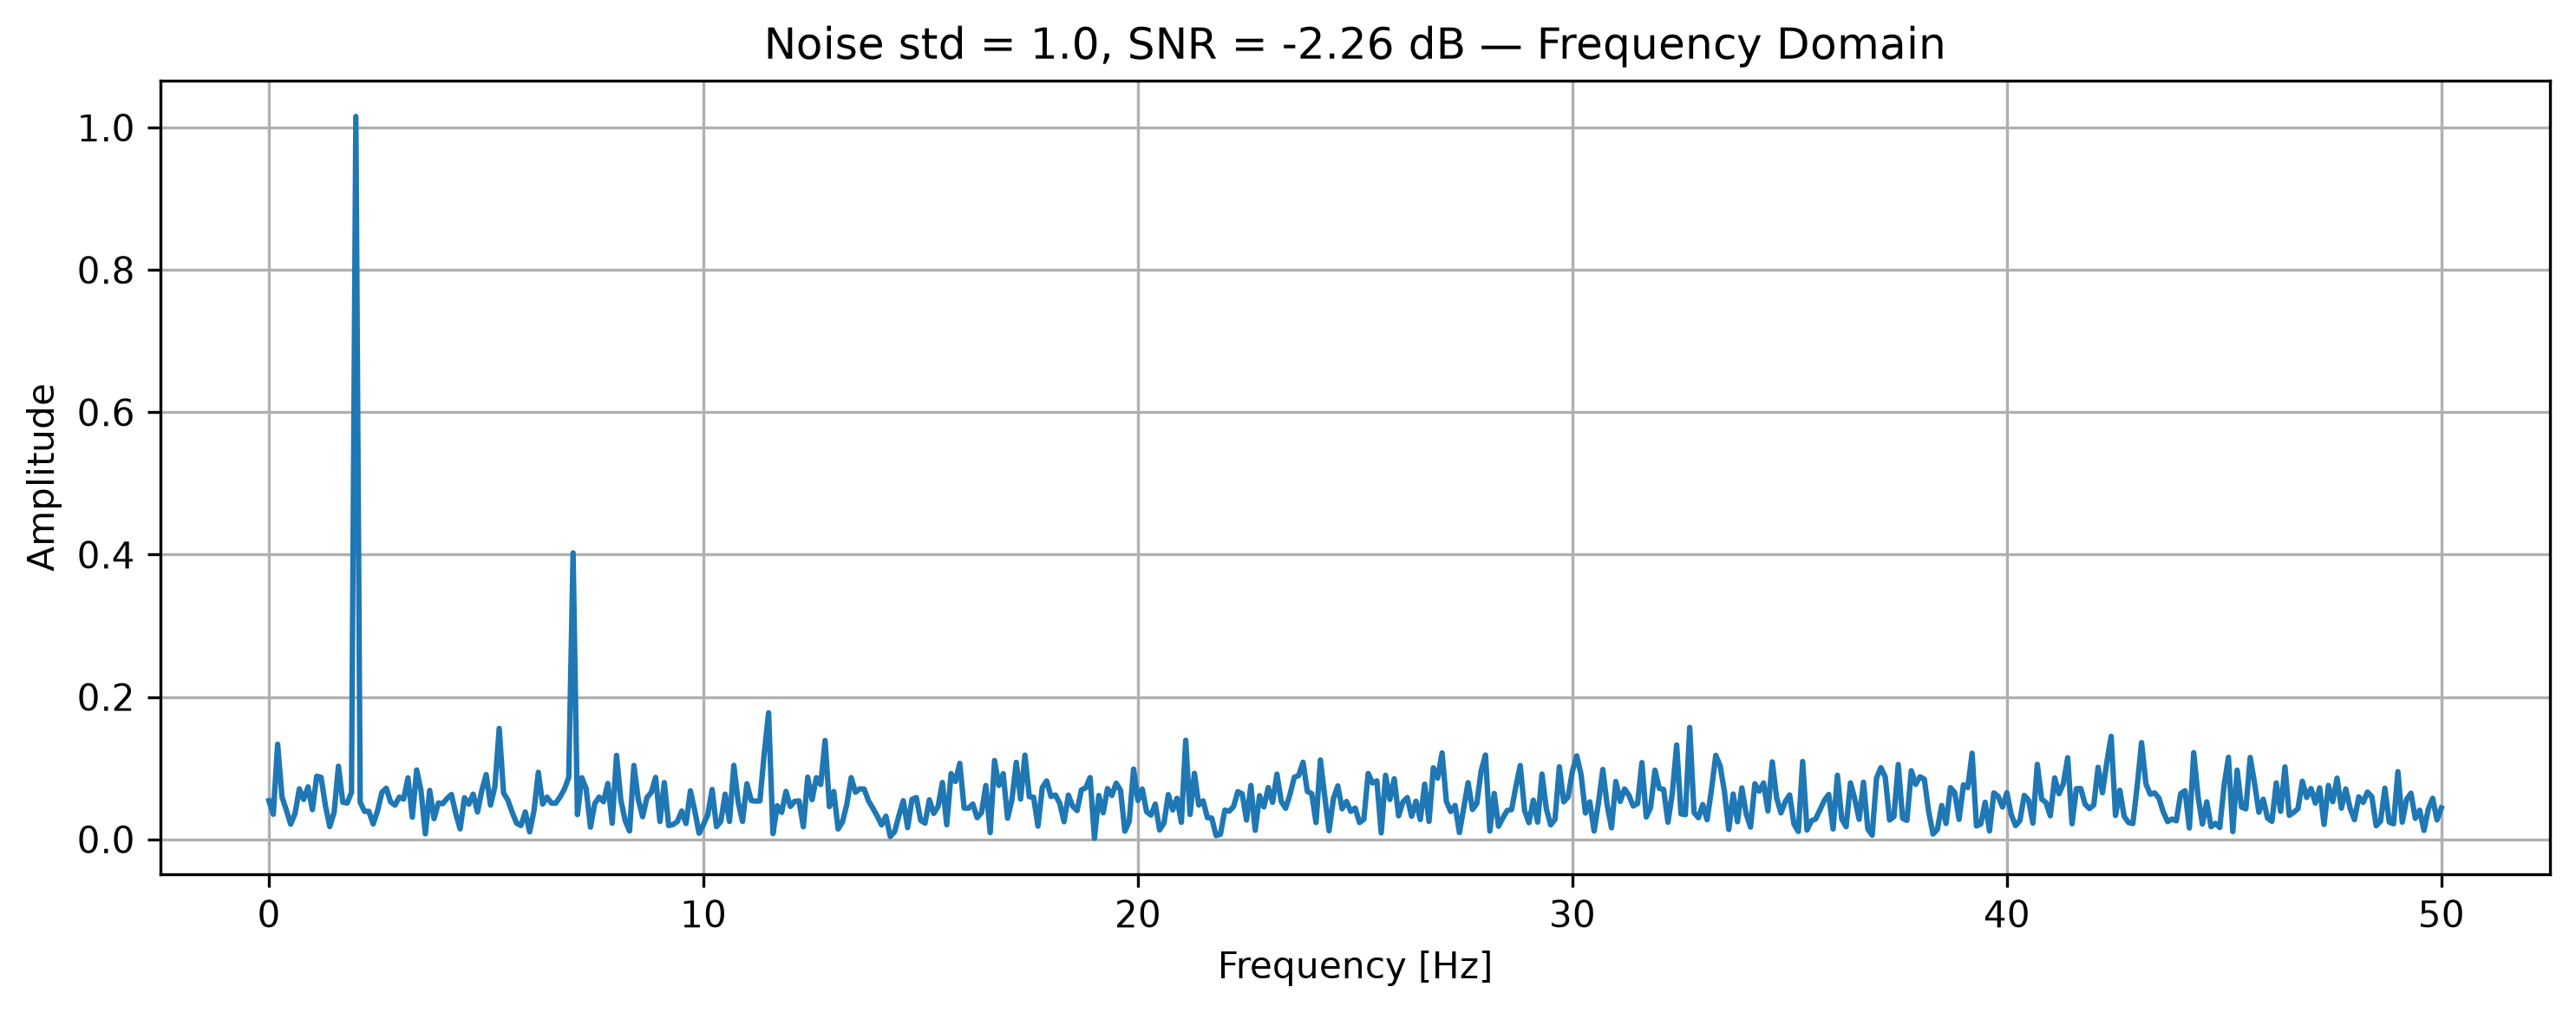
\includegraphics[width=\textwidth]{figures/exp3_sigma_1_0_frequency.png}
        \caption{Frequency domain.}
    \end{subfigure}
    \caption{Noise sensitivity result for \(\sigma = 1.0\).}
\end{figure}

\subsection{Observations}

\begin{itemize}
    \item Noise affected the time-domain signal more visibly than the frequency-domain peaks.
    \item The stronger \SI{2}{Hz} component was more robust against noise.
    \item The weaker \SI{7}{Hz} component was more sensitive to noise.
    \item Increasing noise raised the spectral noise floor.
\end{itemize}

\subsection{Discussion}

The frequency domain can reveal periodic components even when the time-domain signal is visually noisy. However, weak components may become difficult to distinguish from the noise floor.

This is relevant in SHM because higher modes or local vibration effects often have lower amplitudes than the dominant global modes.

% ---------------------------------------------------------
\section{Experiment 4: Duration and Frequency Resolution}

\subsection{Premise}

The fourth experiment studies how total signal duration affects frequency resolution. The sampling frequency is kept constant, while the duration is varied.

\begin{table}[H]
\centering
\caption{Experiment 4 parameters.}
\label{tab:exp4_params}
\begin{tabular}{cccc}
\toprule
Case & Sampling Frequency & Duration & Frequency Resolution \\
\midrule
1 & \SI{100}{Hz} & \SI{2}{s} & \SI{0.5}{Hz} \\
2 & \SI{100}{Hz} & \SI{5}{s} & \SI{0.2}{Hz} \\
3 & \SI{100}{Hz} & \SI{20}{s} & \SI{0.05}{Hz} \\
\bottomrule
\end{tabular}
\end{table}

\subsection{Results}

For the original signal containing \SI{2}{Hz} and \SI{7}{Hz}, all durations identified the main peaks. However, longer durations produced finer frequency spacing and sharper spectral interpretation.

\begin{figure}[H]
    \centering
    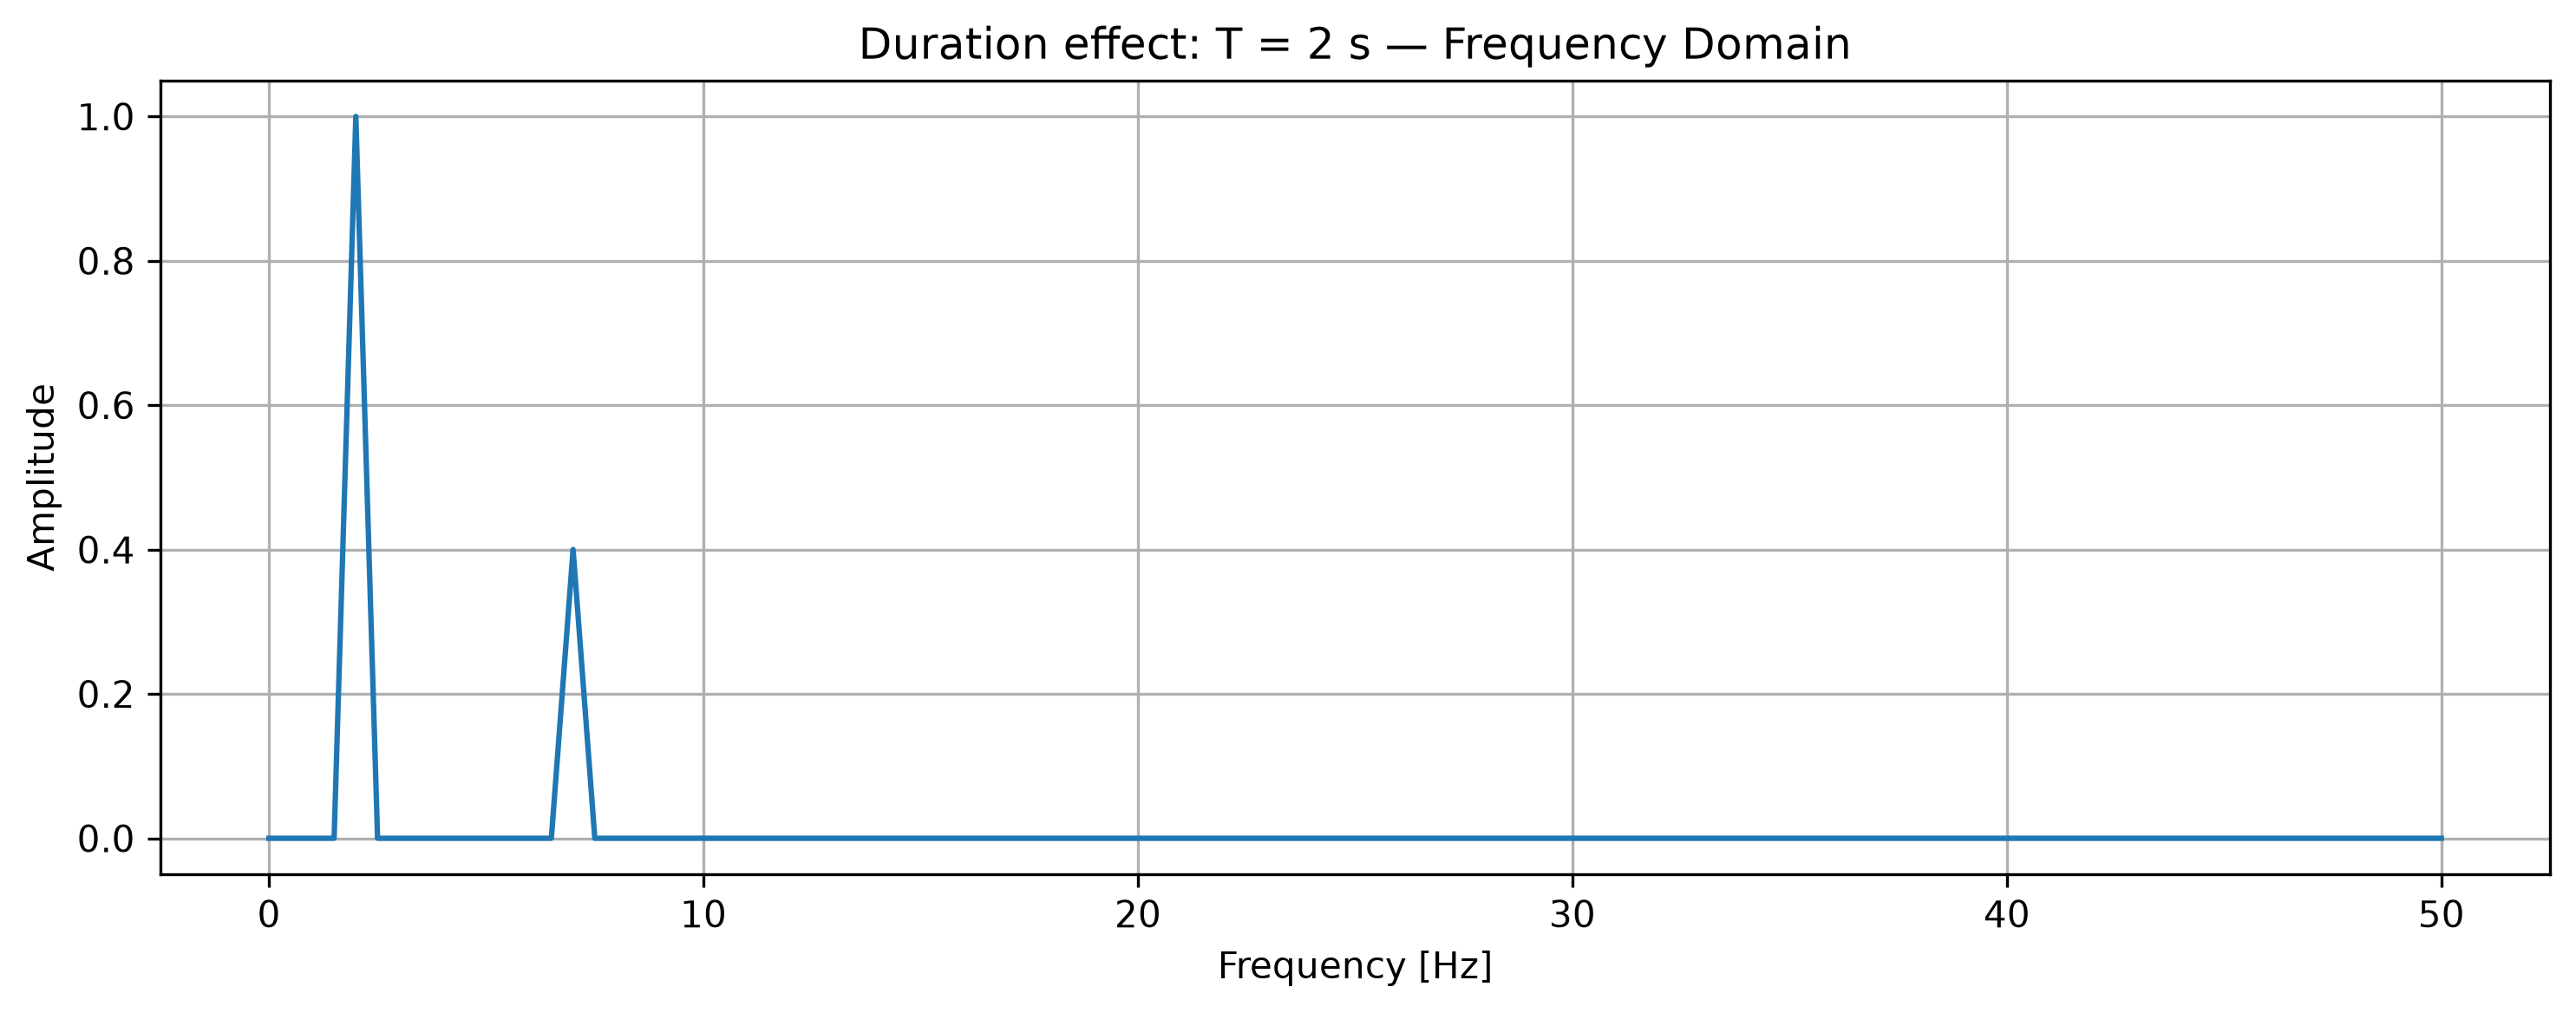
\includegraphics[width=0.92\textwidth]{figures/exp4a_T2_frequency.png}
    \caption{Frequency spectrum with \(\Delta f=\SI{0.5}{Hz}\).}
\end{figure}

\begin{figure}[H]
    \centering
    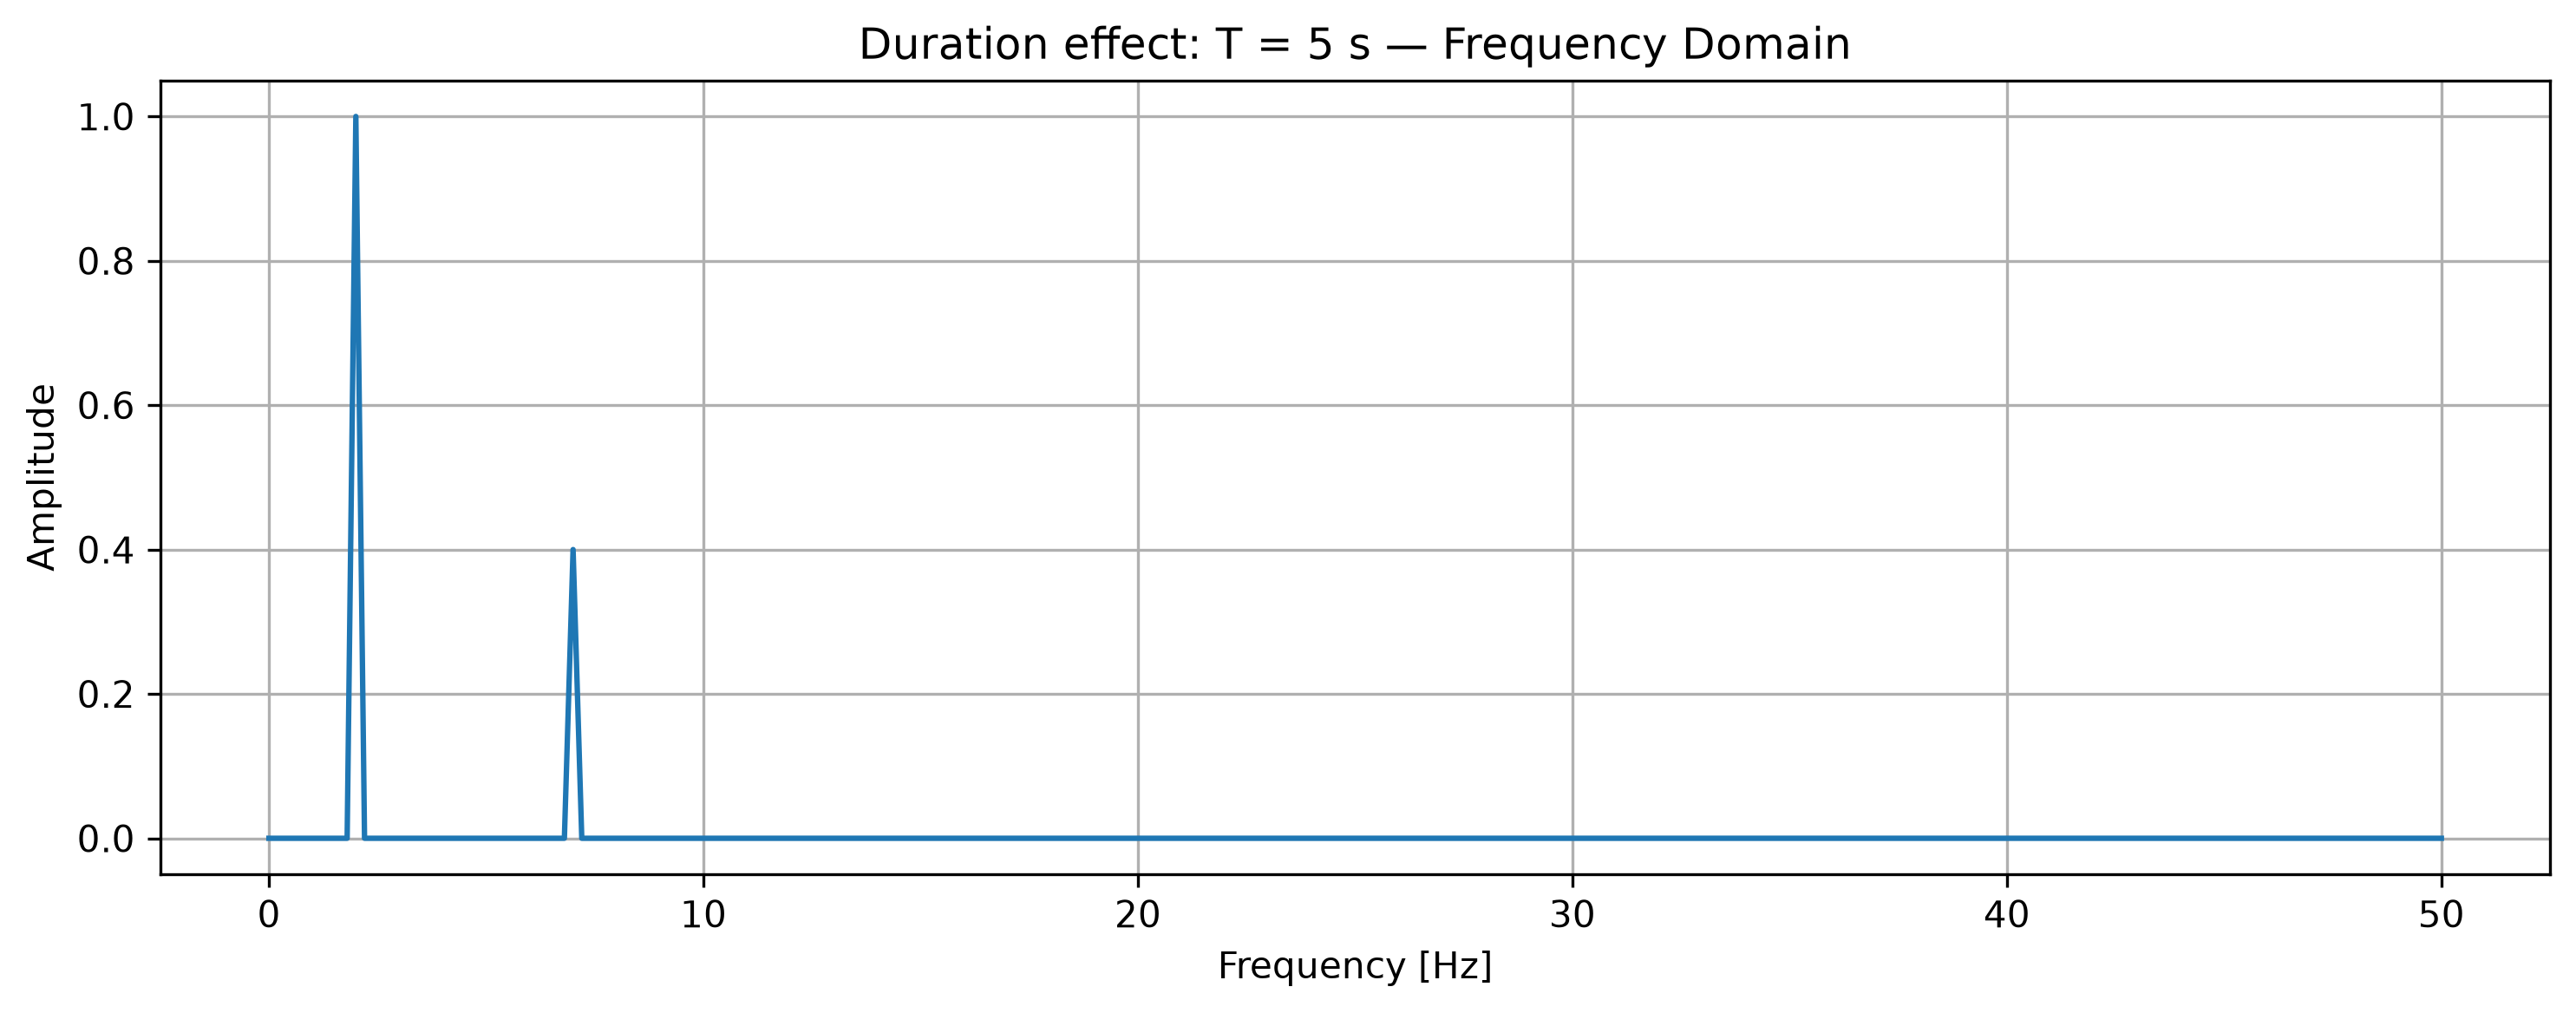
\includegraphics[width=0.92\textwidth]{figures/exp4a_T5_frequency.png}
    \caption{Frequency spectrum with \(\Delta f=\SI{0.2}{Hz}\).}
\end{figure}

\begin{figure}[H]
    \centering
    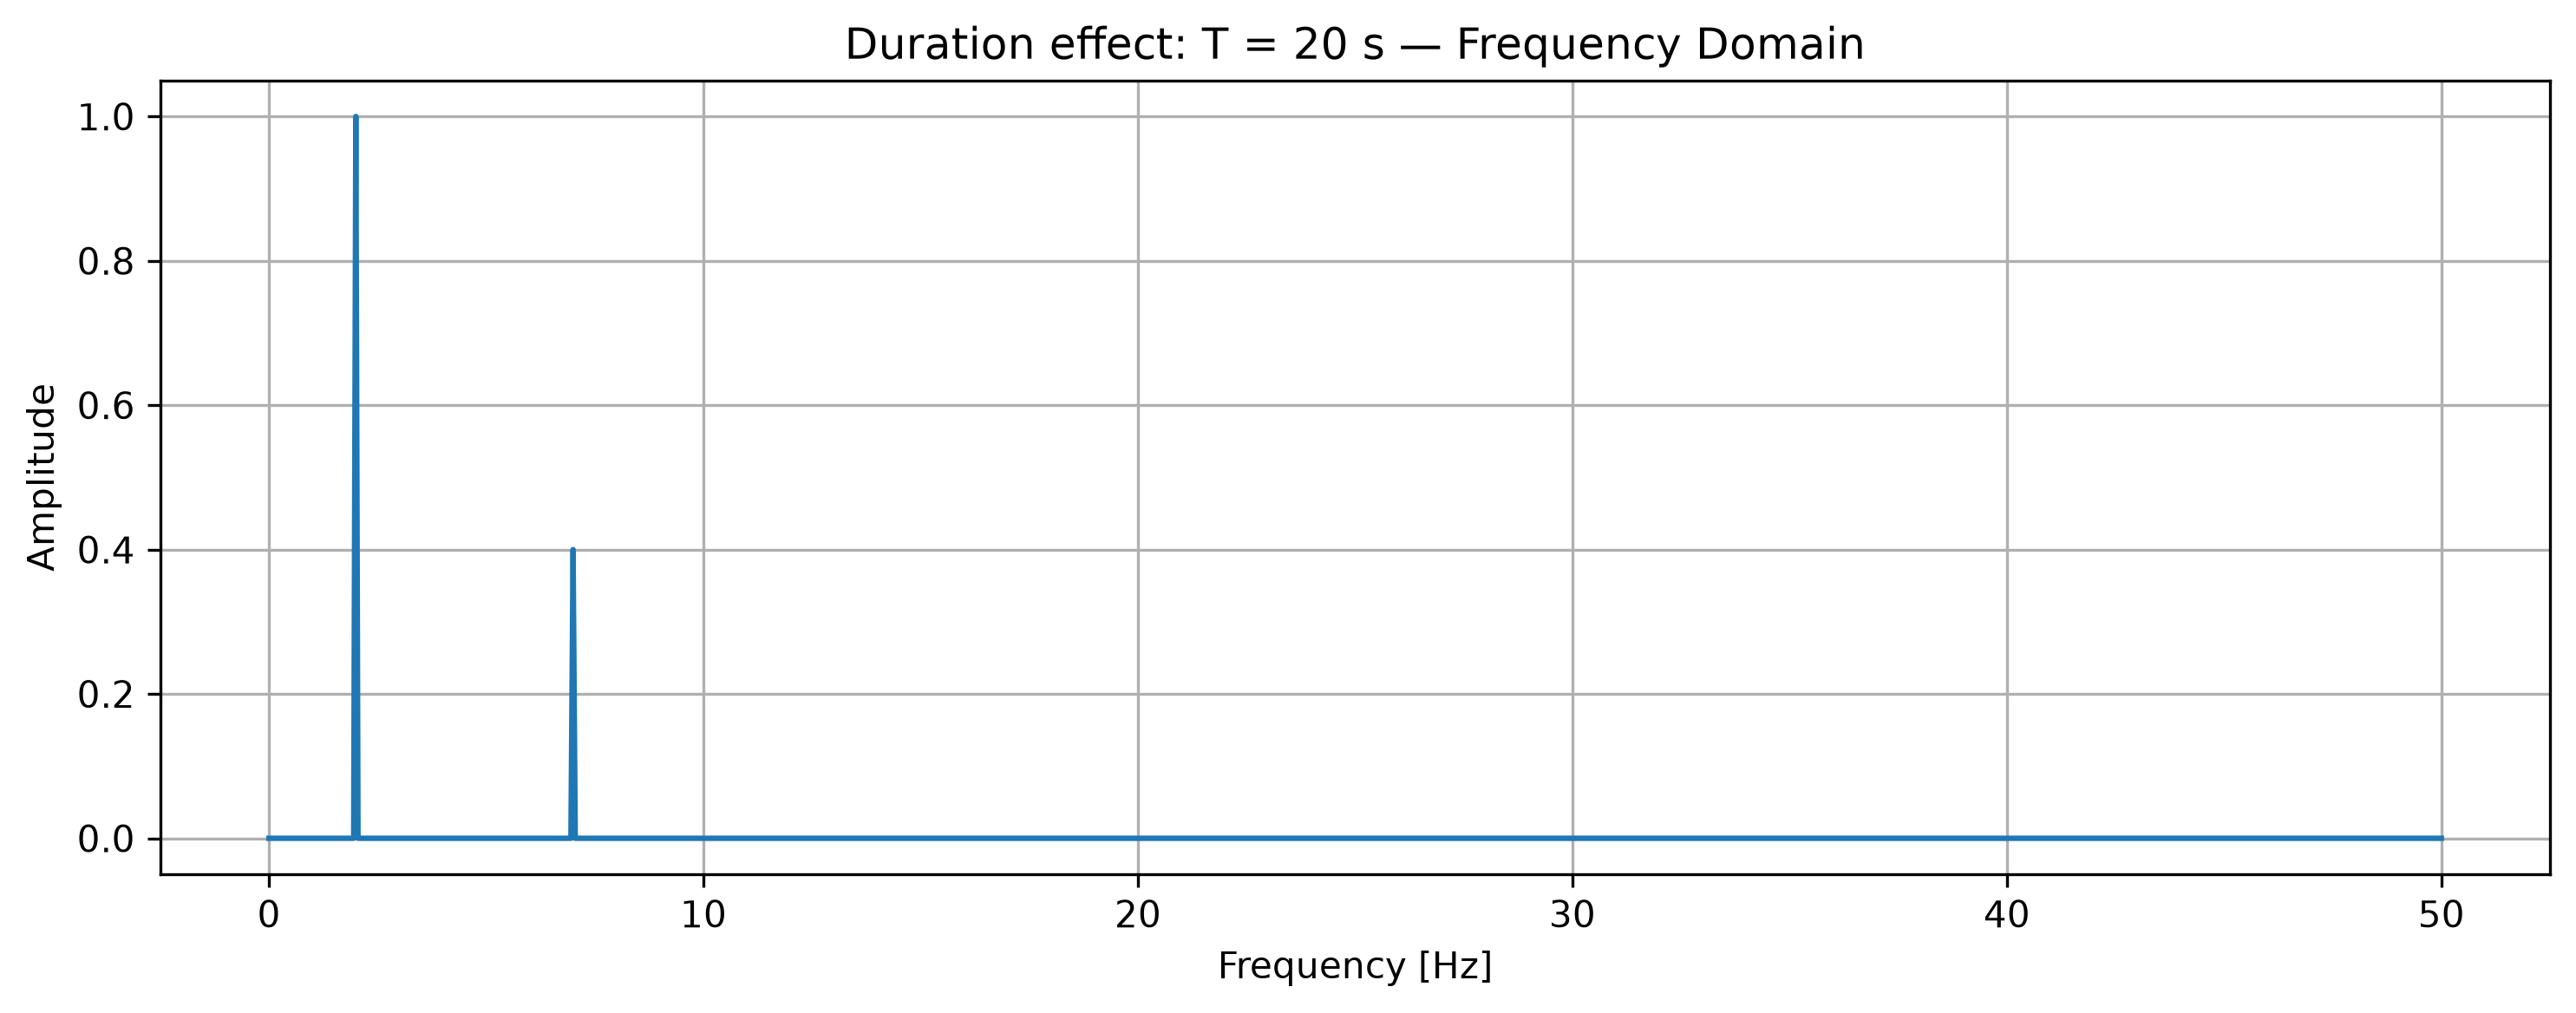
\includegraphics[width=0.92\textwidth]{figures/exp4a_T20_frequency.png}
    \caption{Frequency spectrum with \(\Delta f=\SI{0.05}{Hz}\).}
\end{figure}

\subsection{Close-Frequency Case}

To highlight the effect of duration, a second case was tested using close frequencies:

\begin{equation}
x(t) = 1.0\sin(2\pi(2.0)t) + 0.7\sin(2\pi(2.3)t)
\end{equation}

The frequency separation is

\begin{equation}
\Delta f_{\text{modes}} = 2.3 - 2.0 = \SI{0.3}{Hz}
\end{equation}

\begin{figure}[H]
    \centering
    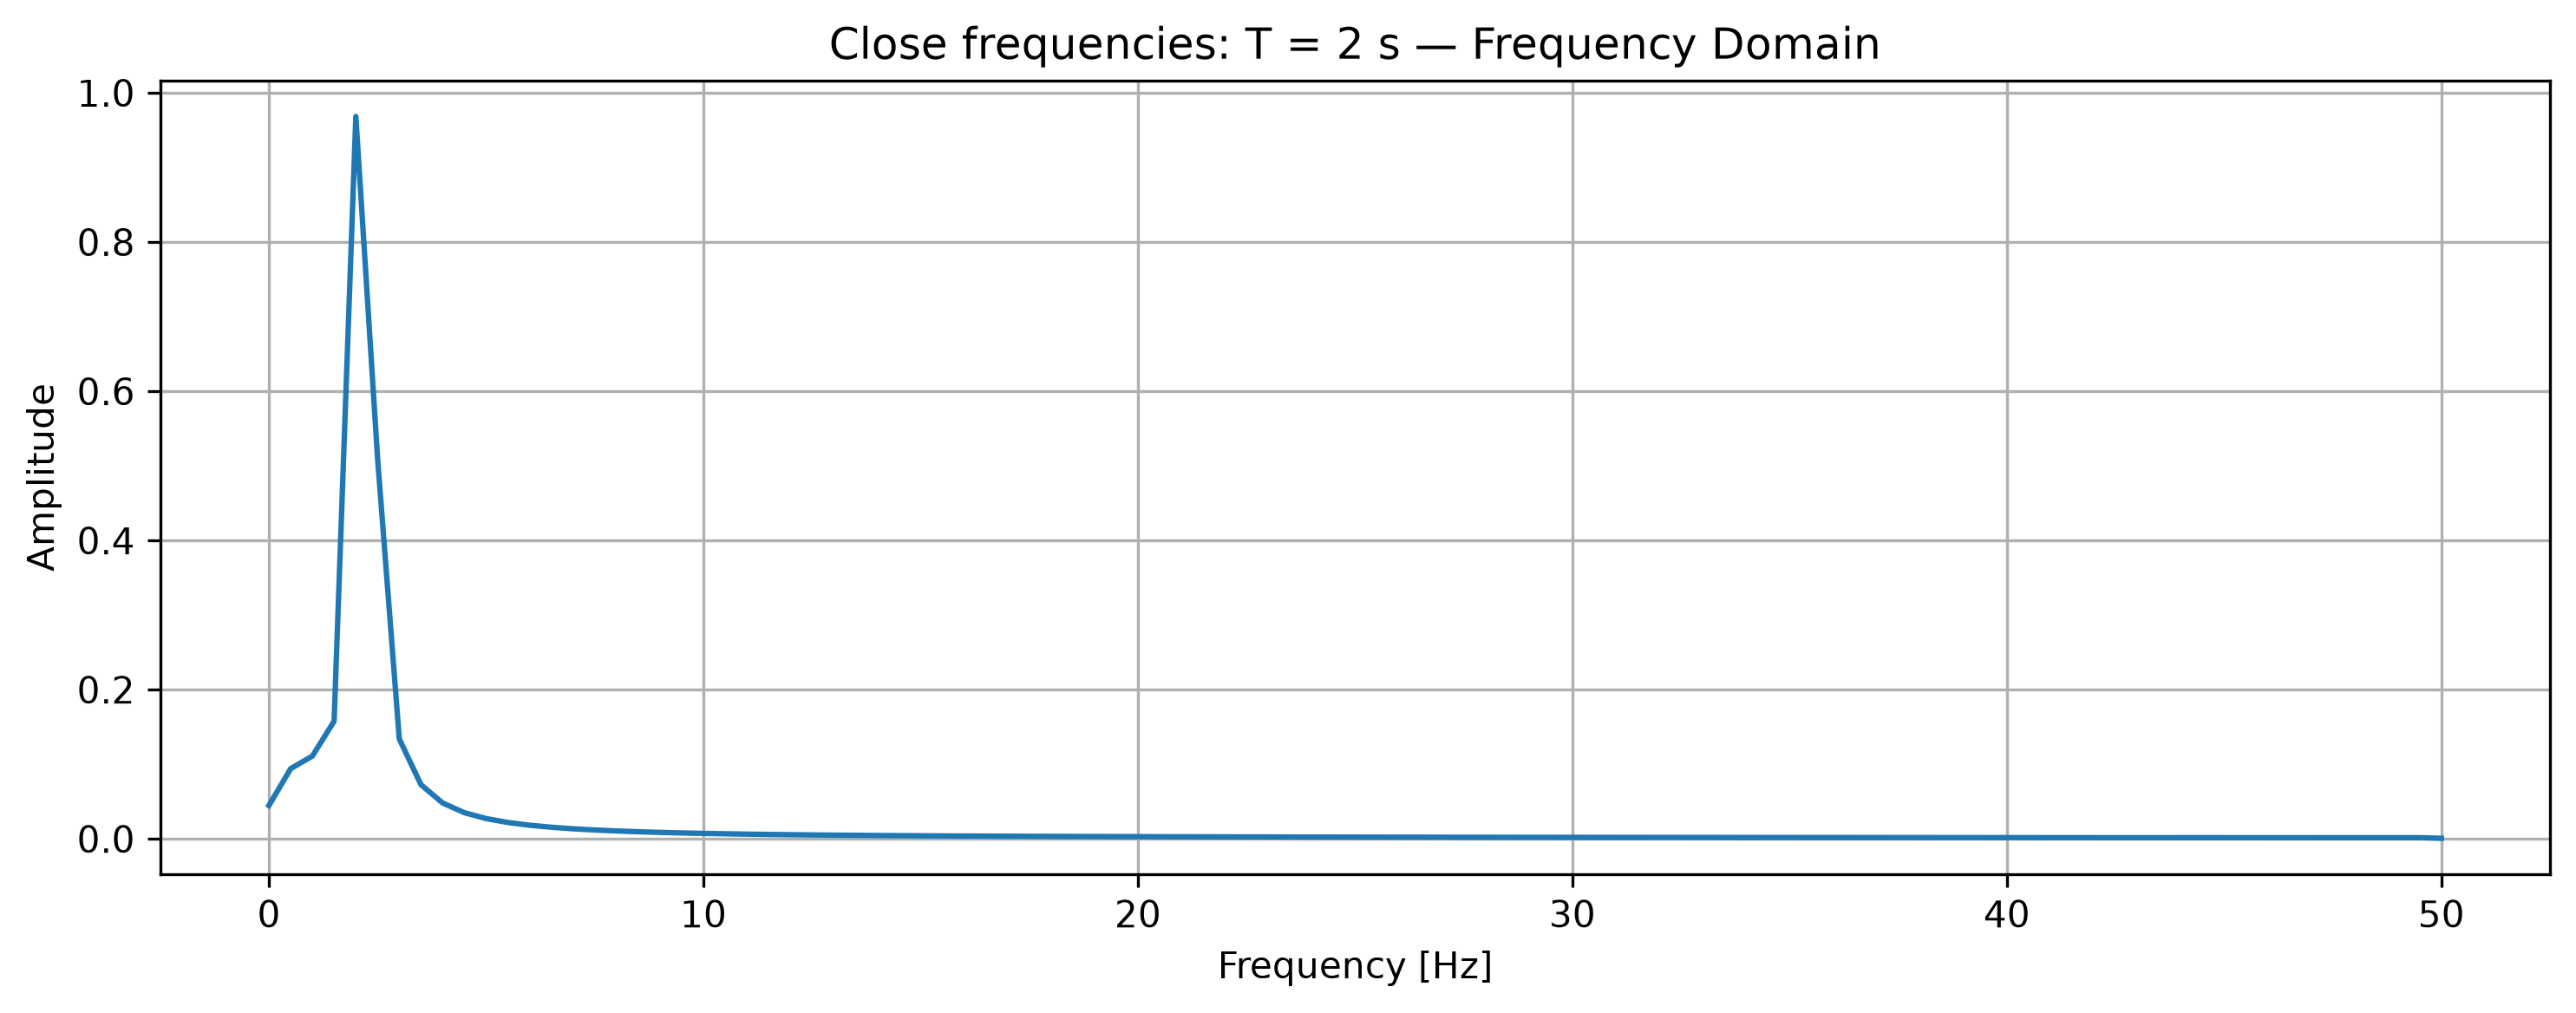
\includegraphics[width=0.92\textwidth]{figures/exp4b_T2_frequency.png}
    \caption{Close-frequency case with short duration.}
\end{figure}

\begin{figure}[H]
    \centering
    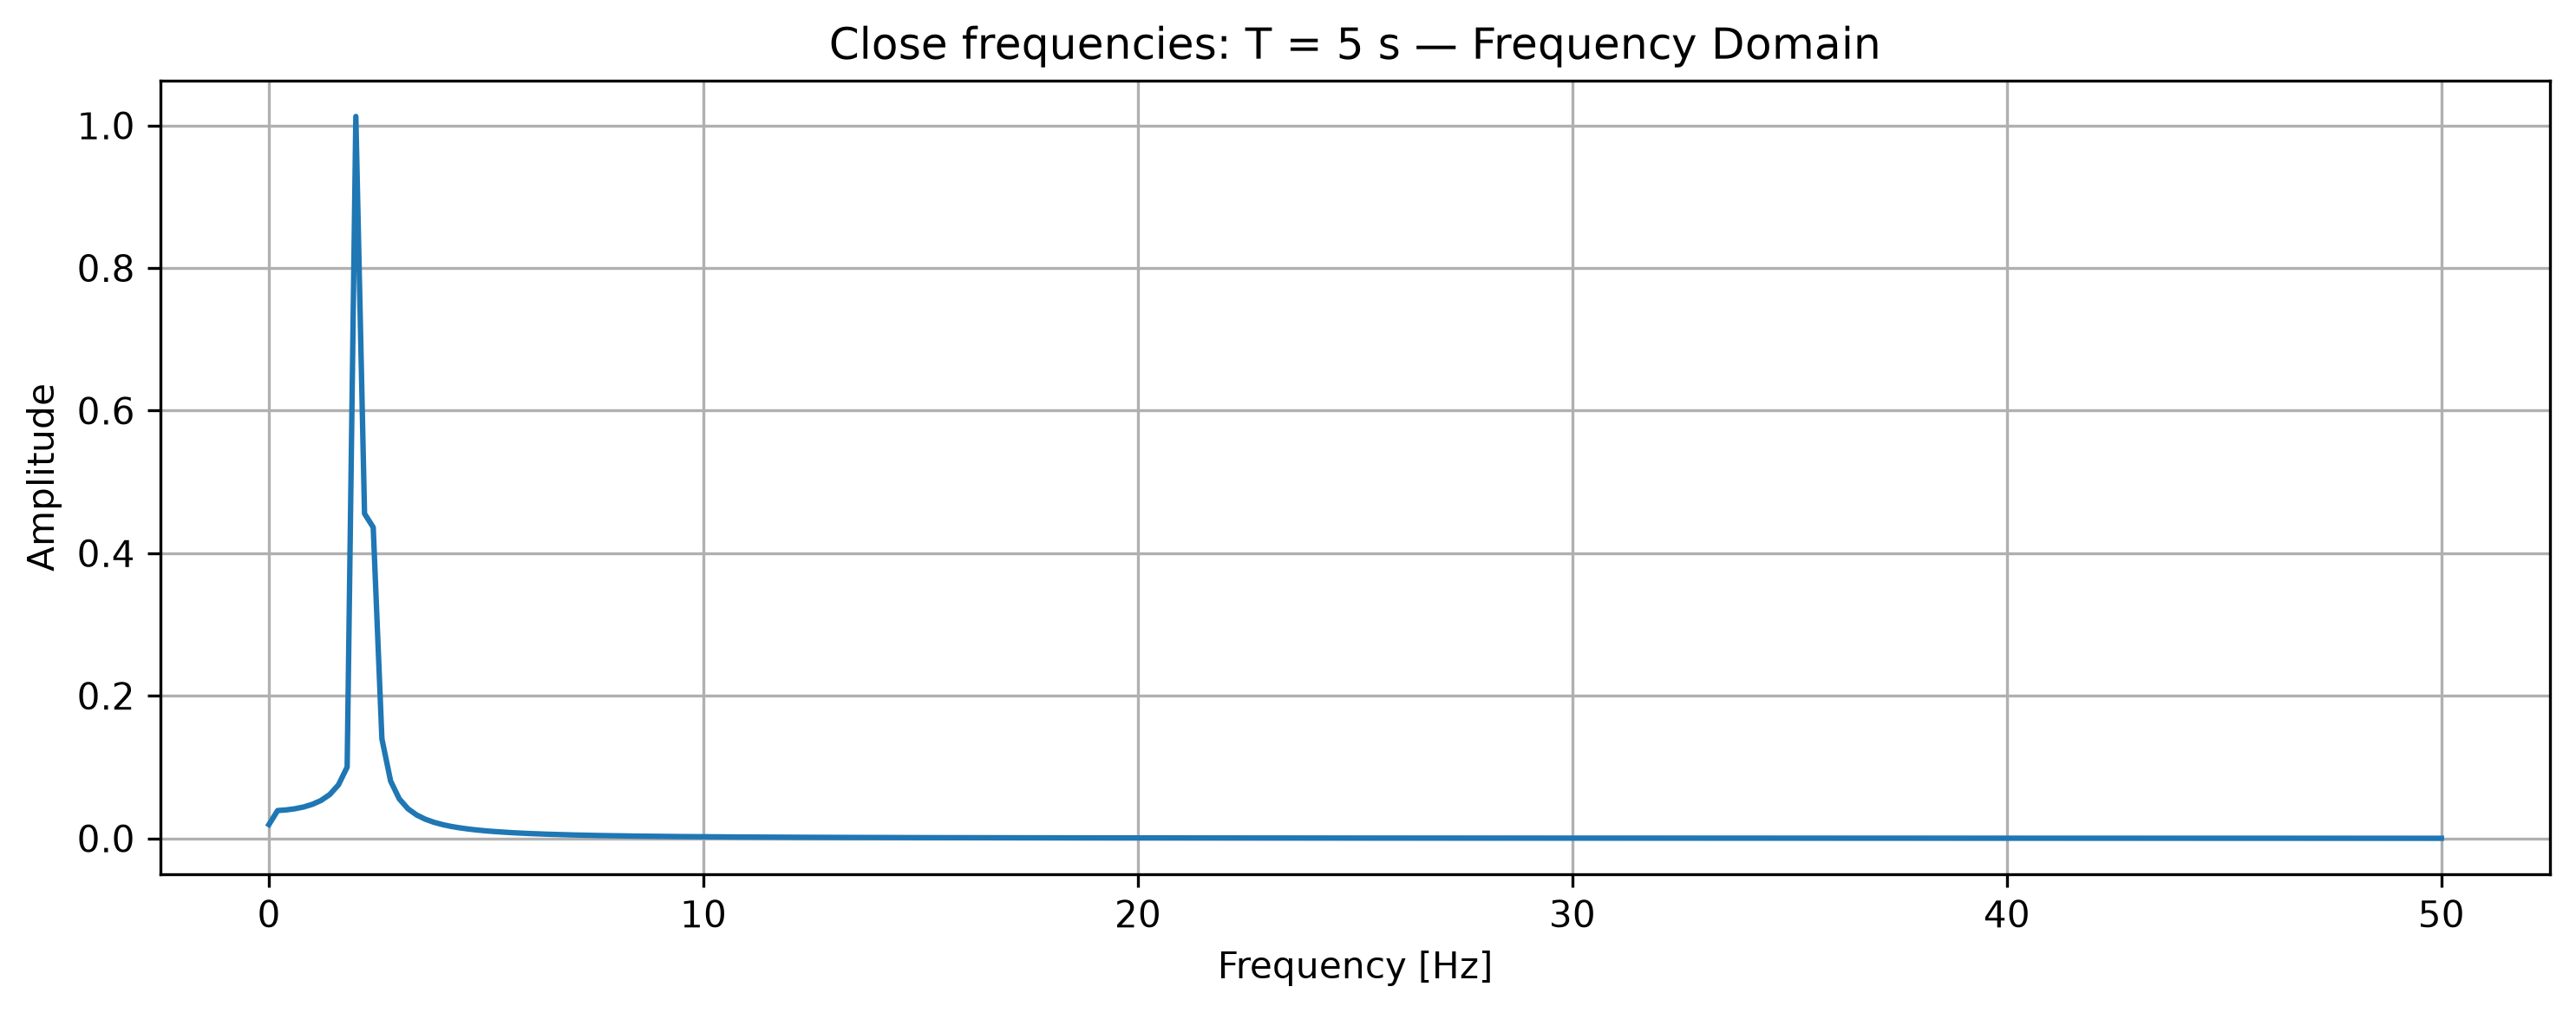
\includegraphics[width=0.92\textwidth]{figures/exp4b_T5_frequency.png}
    \caption{Close-frequency case with intermediate duration.}
\end{figure}

\begin{figure}[H]
    \centering
    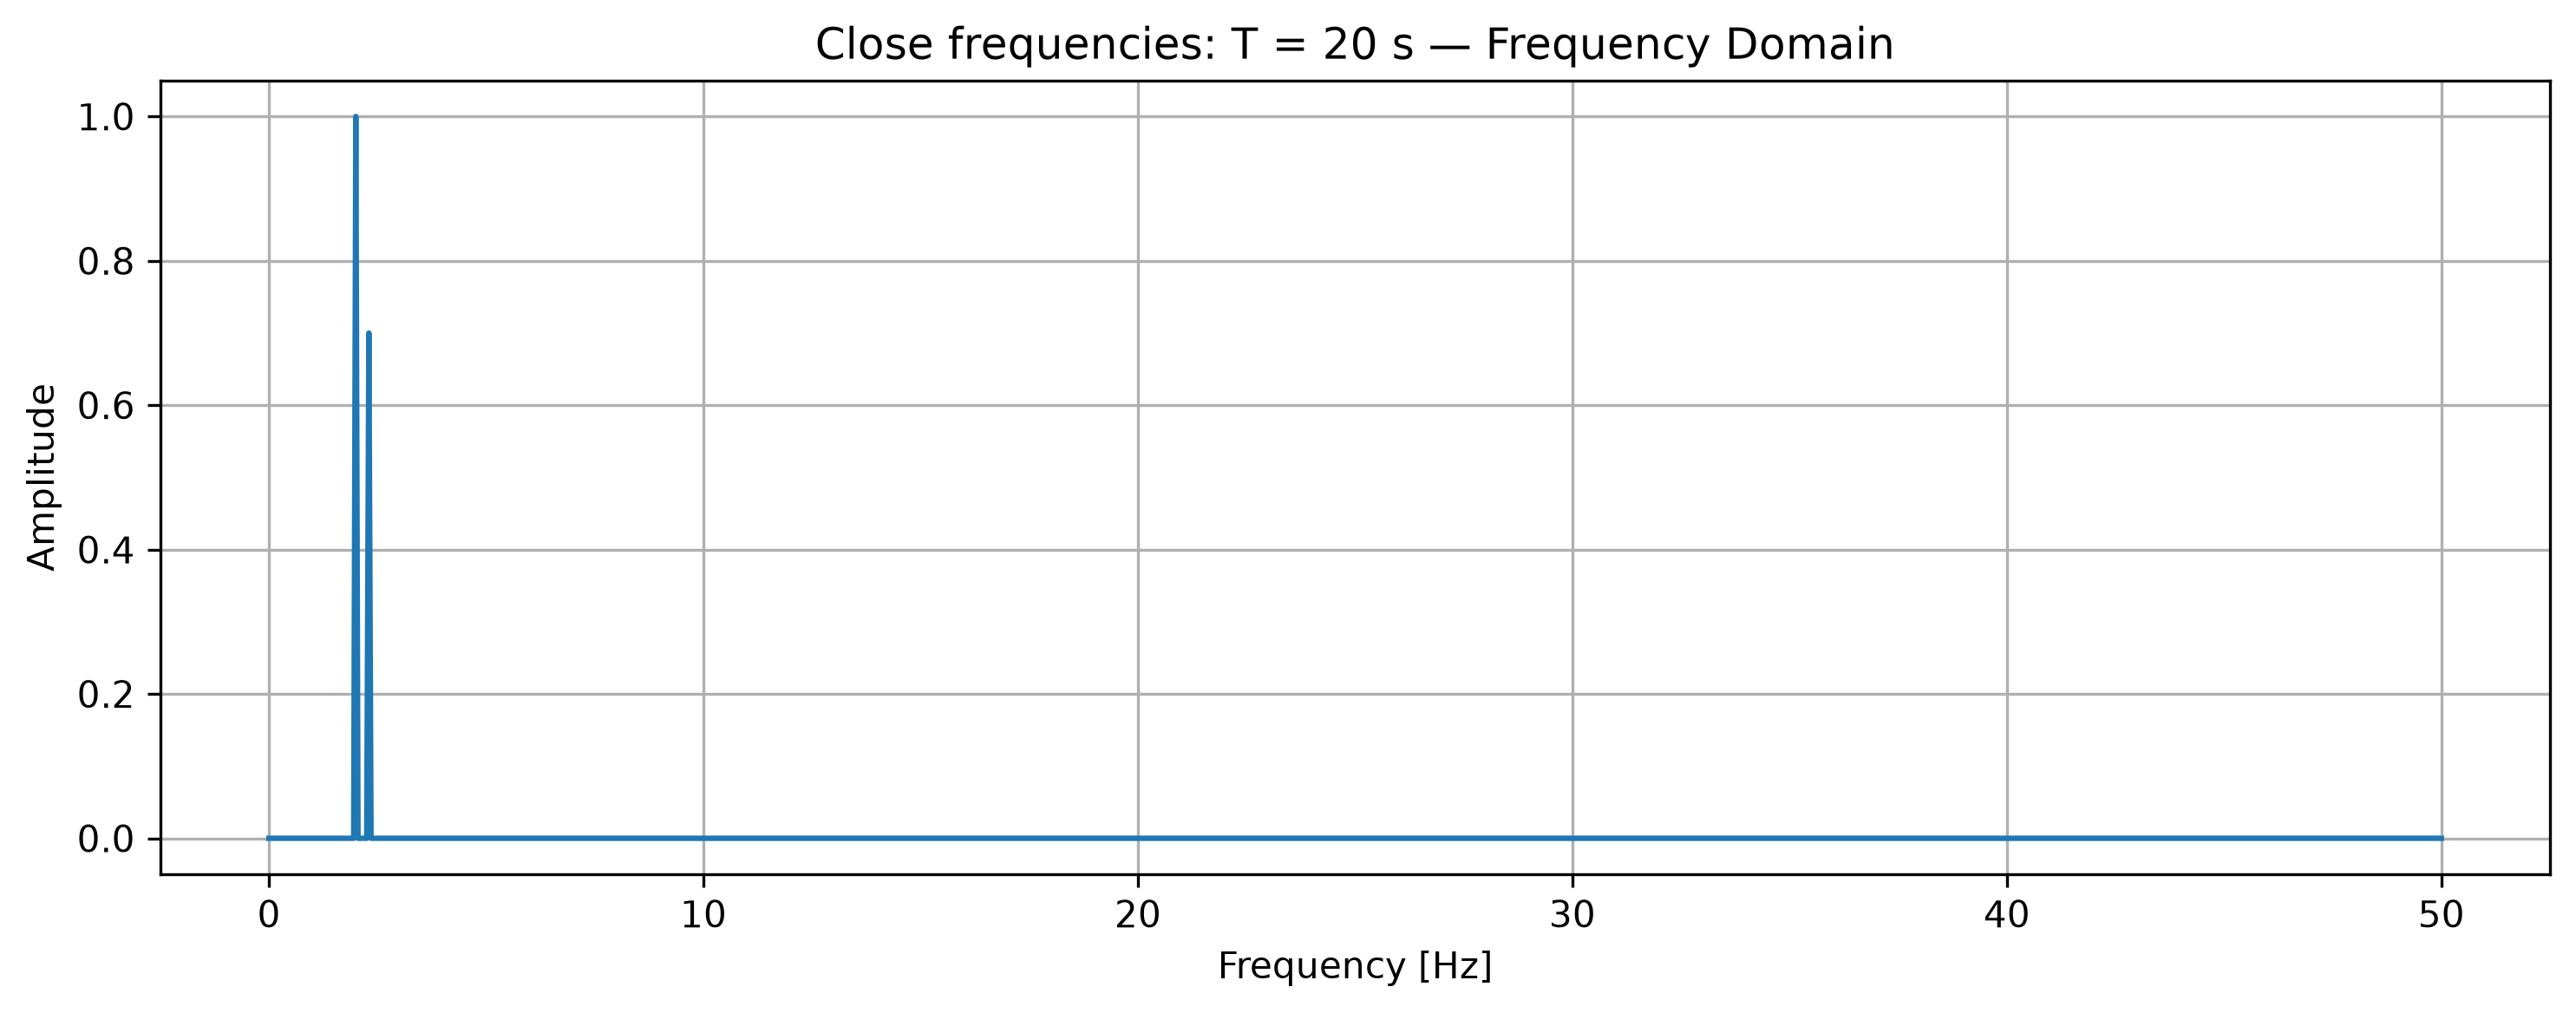
\includegraphics[width=0.92\textwidth]{figures/exp4b_T20_frequency.png}
    \caption{Close-frequency case with long duration.}
\end{figure}

\subsection{Observations}

\begin{itemize}
    \item Increasing duration reduced the FFT frequency spacing.
    \item Short duration produced coarse spectral resolution.
    \item Long duration improved the separation of close frequency components.
    \item Sampling frequency and duration control different aspects of the analysis.
\end{itemize}

\subsection{Discussion}

Sampling frequency controls the highest frequency that can be captured without aliasing. Signal duration controls how precisely the frequency axis is resolved.

This distinction is important in modal identification. Closely spaced modes require sufficiently long measurement records.

% ---------------------------------------------------------
\section{Experiment 5: Spectral Leakage and Windowing}

\subsection{Premise}

The fifth experiment studies spectral leakage. Even when the sampling frequency is adequate, leakage can occur if the signal frequency does not align with an FFT frequency bin.

For a duration of \(T=\SI{10}{s}\), the FFT bin spacing is

\begin{equation}
\Delta f = \frac{1}{10} = \SI{0.1}{Hz}
\end{equation}

A frequency of \SI{2.0}{Hz} lies exactly on an FFT bin. A frequency of \SI{2.25}{Hz} lies between FFT bins.

\begin{table}[H]
\centering
\caption{Experiment 5 parameters.}
\label{tab:exp5_params}
\begin{tabular}{cccc}
\toprule
Case & Frequency & Duration & Expected Behavior \\
\midrule
A & \SI{2.0}{Hz} & \SI{10}{s} & Minimal leakage \\
B & \SI{2.25}{Hz} & \SI{10}{s} & Leakage expected \\
C & \SI{2.25}{Hz} & \SI{10}{s} & Hann window applied \\
\bottomrule
\end{tabular}
\end{table}

\subsection{Results}

For the \SI{2.0}{Hz} signal, the FFT showed a concentrated peak because the frequency aligned with an FFT bin.

For the \SI{2.25}{Hz} signal, the FFT energy spread into neighboring bins because the frequency did not align exactly with the FFT bin spacing.

After applying a Hann window, distant leakage was reduced, but the main peak became wider.

\begin{figure}[H]
    \centering
    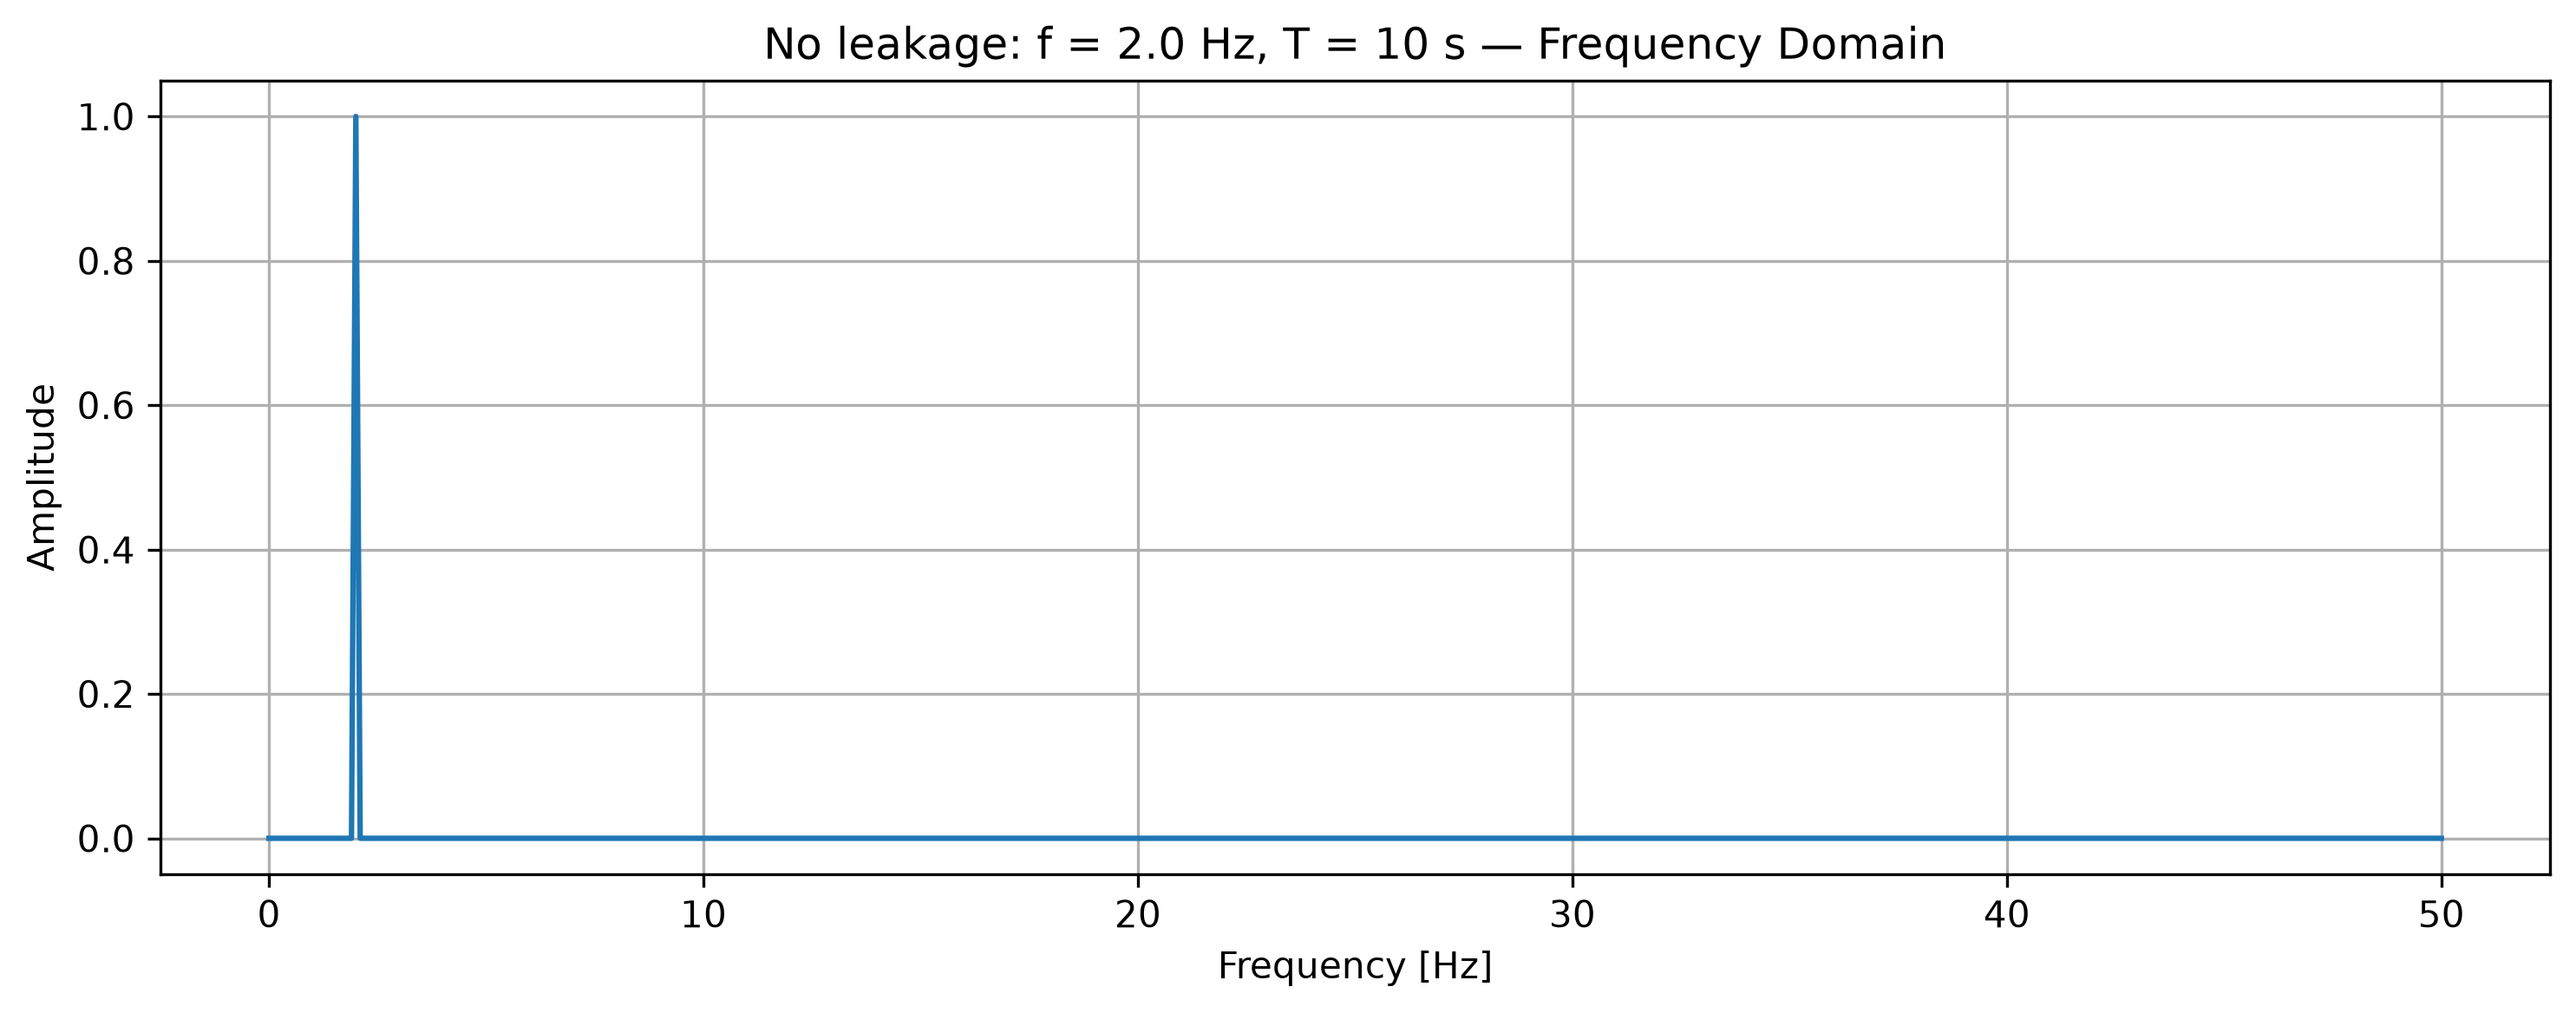
\includegraphics[width=0.92\textwidth]{figures/exp5a_frequency.png}
    \caption{Frequency aligned with FFT bin.}
\end{figure}

\begin{figure}[H]
    \centering
    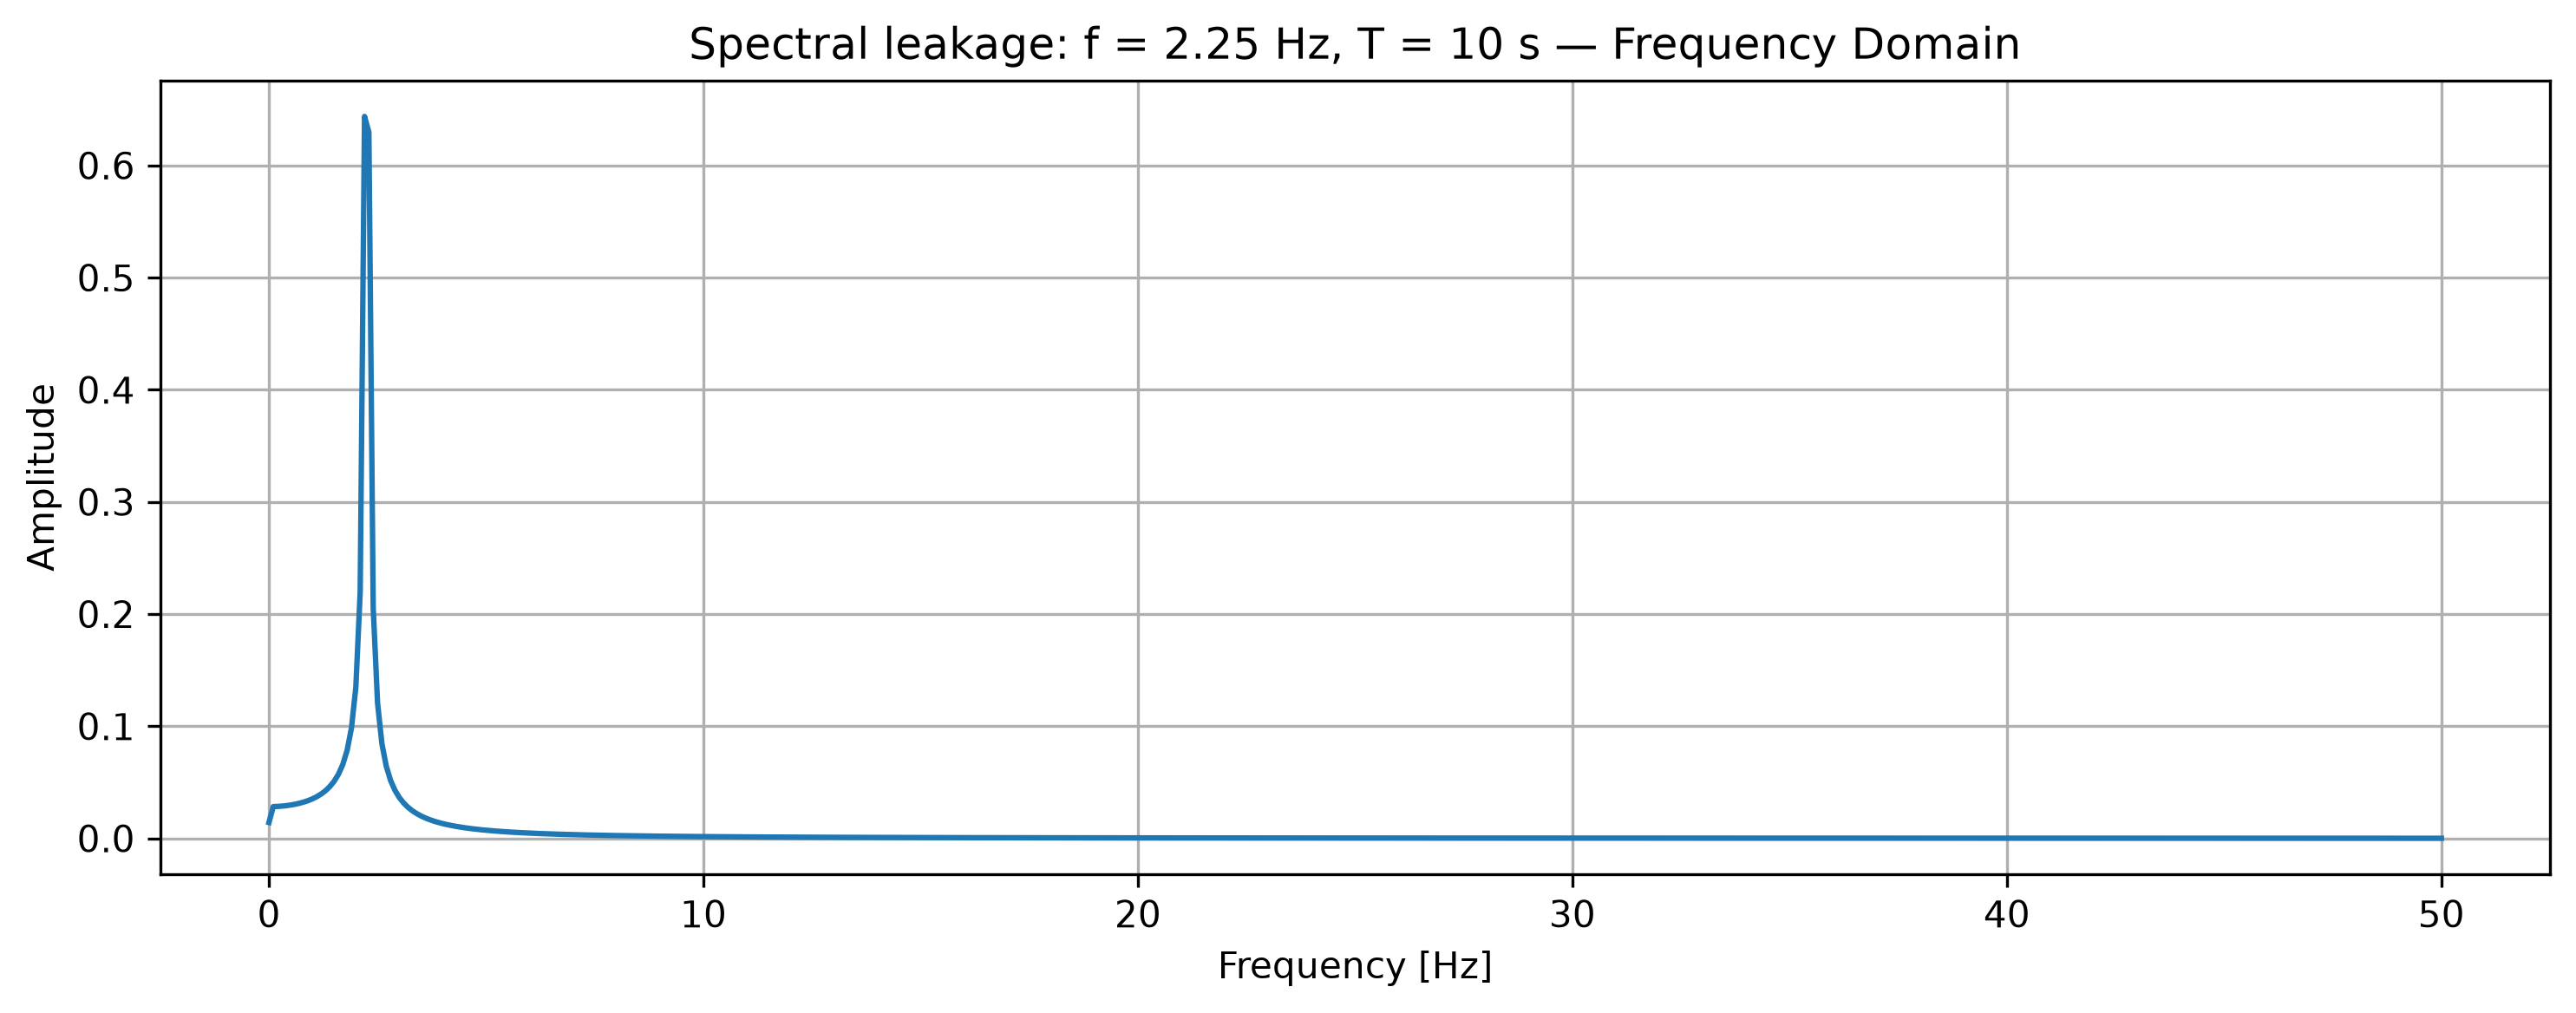
\includegraphics[width=0.92\textwidth]{figures/exp5b_frequency.png}
    \caption{Spectral leakage for frequency between FFT bins.}
\end{figure}

\begin{figure}[H]
    \centering
    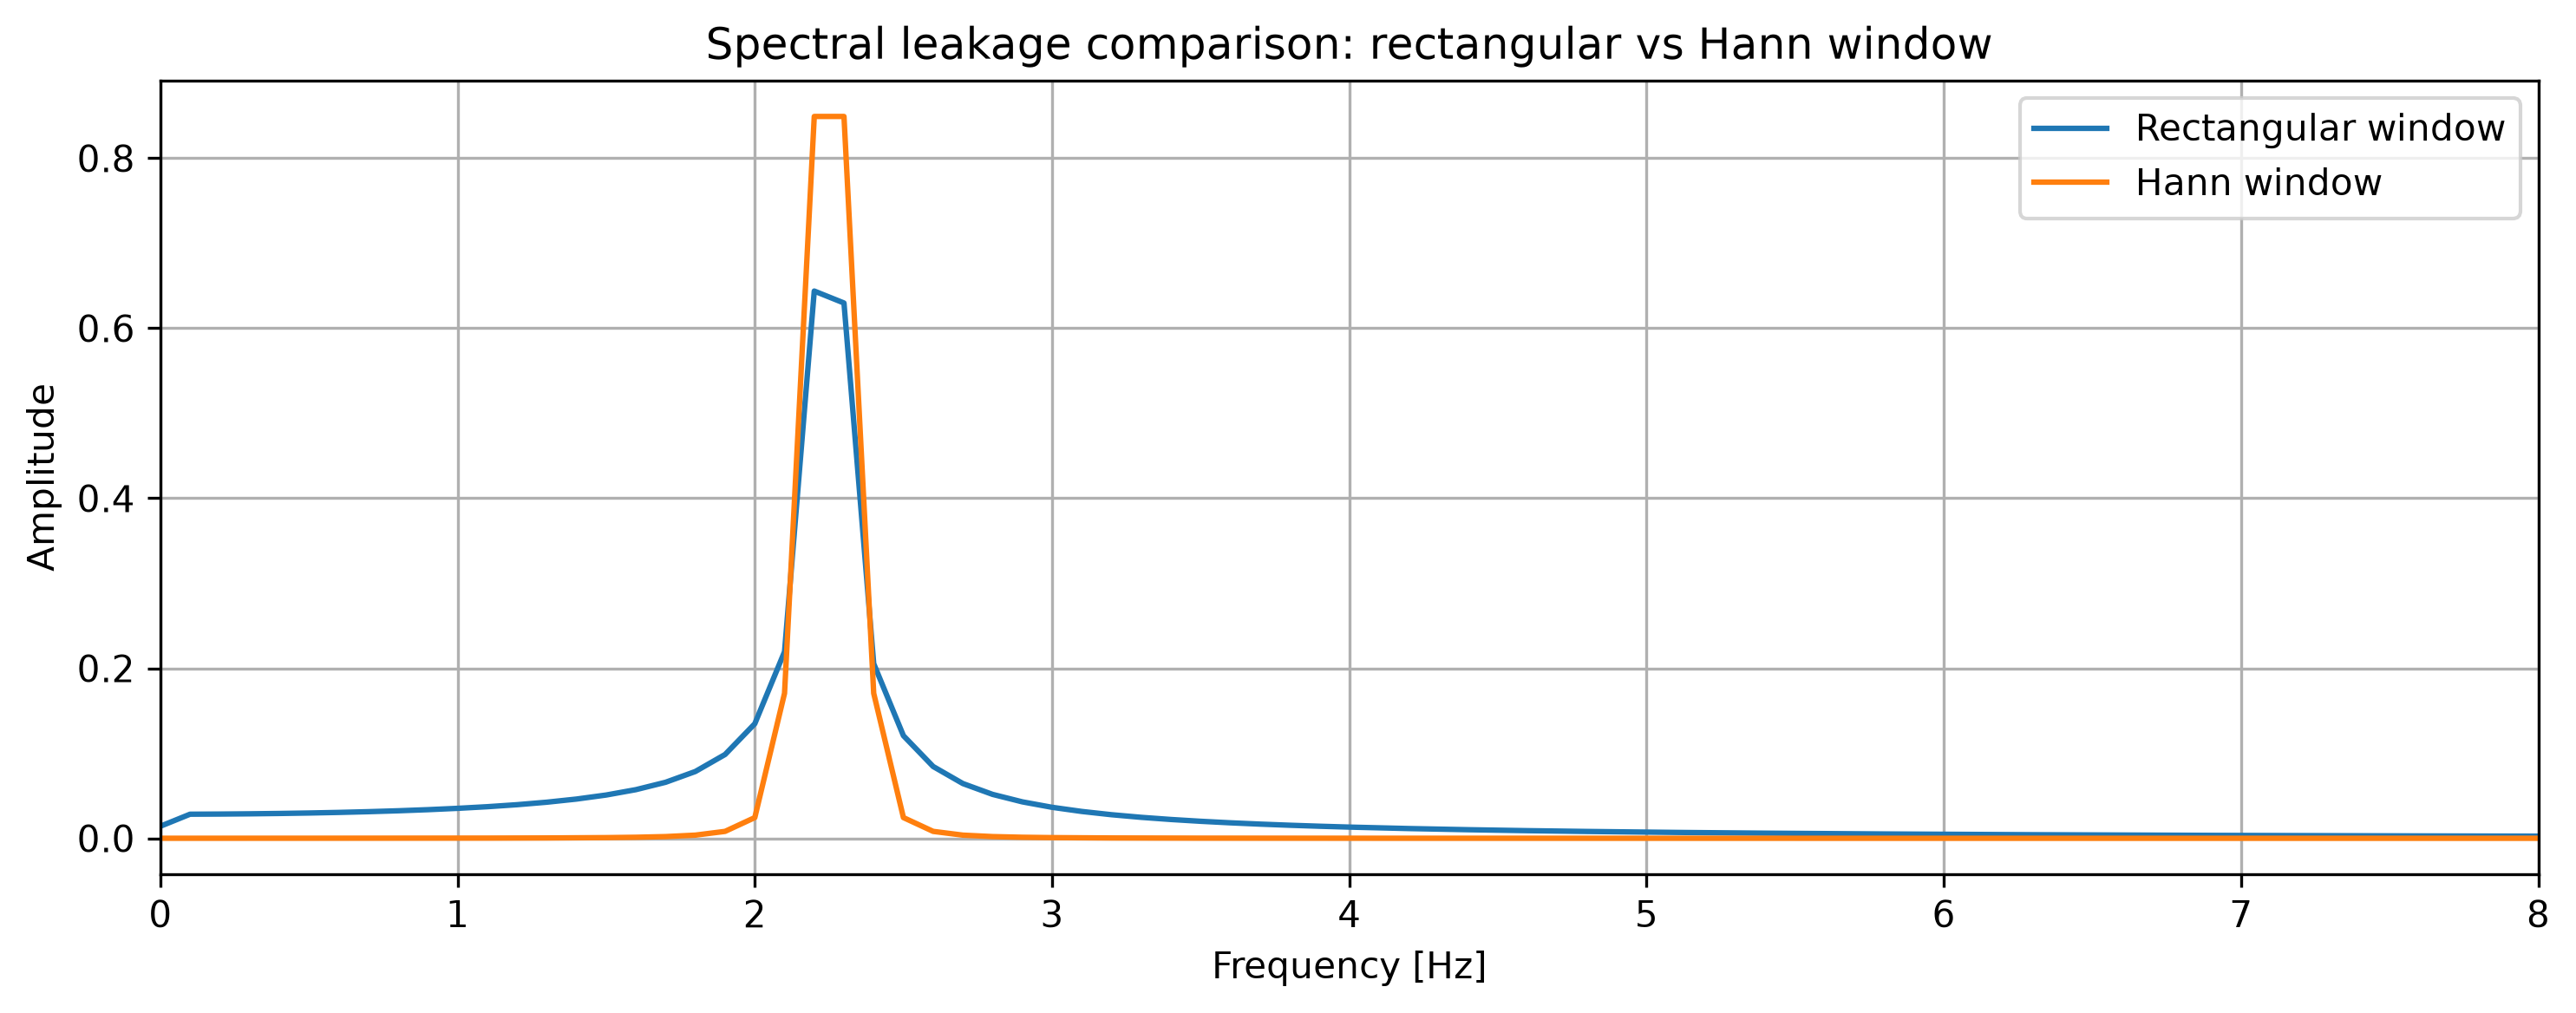
\includegraphics[width=0.92\textwidth]{figures/exp5c_window_comparison.png}
    \caption{Effect of Hann window on spectral leakage.}
\end{figure}

\subsection{Observations}

\begin{itemize}
    \item A bin-centered sinusoid produced a clean FFT peak.
    \item A non-bin-centered sinusoid caused spectral leakage.
    \item The Hann window reduced leakage away from the main peak.
    \item Windowing widened the main lobe of the spectrum.
\end{itemize}

\subsection{Discussion}

Spectral leakage is not caused by poor sampling alone. It is caused by the finite duration of the record and the mismatch between the signal frequency and FFT bin locations.

For measured vibration data, modal frequencies rarely align exactly with FFT bins. Windowing is therefore a practical tool for improving spectral interpretation.

% ---------------------------------------------------------
\section{Structural Health Monitoring Example}

Consider an instrumented tall building with two close lateral vibration modes:

\begin{equation}
f_1 = \SI{0.85}{Hz}
\end{equation}

\begin{equation}
f_2 = \SI{0.92}{Hz}
\end{equation}

The modal separation is

\begin{equation}
\Delta f_{\text{modes}} = 0.92 - 0.85 = \SI{0.07}{Hz}
\end{equation}

To resolve these two modes, the measurement duration should satisfy approximately

\begin{equation}
T > \frac{1}{0.07}
\end{equation}

\begin{equation}
T > \SI{14.3}{s}
\end{equation}

In practice, a longer duration is preferred because ambient vibration data contains noise, operational variation, and possible nonstationary effects.

This example shows why SHM measurements require both adequate sampling frequency and adequate record duration.

% ---------------------------------------------------------
\section{Summary of Results}

\begin{table}[H]
\centering
\caption{Summary of Stage 1 experiments.}
\label{tab:summary}
\begin{tabular}{p{0.22\textwidth} p{0.32\textwidth} p{0.34\textwidth}}
\toprule
Experiment & Main Concept & Engineering Observation \\
\midrule
Clean signal & FFT identification & Known frequency components were recovered correctly. \\
Aliasing & Nyquist criterion & Undersampling produced a false lower-frequency peak. \\
Noise sensitivity & SNR and noise floor & Strong components remained visible; weak components became harder to detect. \\
Duration effect & Frequency resolution & Longer records improved frequency resolution. \\
Close frequencies & Modal separation & Closely spaced peaks required longer duration to separate. \\
Windowing & Spectral leakage & Hann window reduced leakage but widened the main peak. \\
\bottomrule
\end{tabular}
\end{table}

% ---------------------------------------------------------

\begin{itemize}
    \item The sampling frequency should be selected based on the highest expected physical frequency.
    \item The Nyquist frequency defines the theoretical upper limit of recoverable frequency content.
    \item A clean FFT peak is not automatically physically correct; aliasing must be checked first.
    \item The total record duration controls frequency resolution.
    \item Weak modal components are more vulnerable to noise than dominant components.
    \item Windowing is useful for finite measured records but changes the spectral shape.
    \item For SHM applications, frequency-domain interpretation should always consider sampling rate, duration, noise level, and windowing.
\end{itemize}

% ---------------------------------------------------------
\section{Conclusion}

This stage established the basic signal-processing workflow for synthetic vibration signals. A multi-sinusoidal vibration signal was generated and analyzed under different sampling and noise conditions.

The experiments demonstrated that adequate sampling is required to avoid aliasing, while sufficient signal duration is required to improve frequency resolution. Noise sensitivity showed that strong vibration components can remain identifiable in the frequency domain even when the time-domain signal becomes visually unclear. Spectral leakage and windowing demonstrated that finite signal records require careful interpretation.

These concepts form the foundation for later stages involving FFT-based modal identification, filtering, short-time Fourier transform analysis, and vibration-based structural health monitoring.

% ---------------------------------------------------------
\section*{Appendix: Implementation Notes}

The signal was generated numerically using a discrete time vector:

\begin{equation}
t_n = n\Delta t
\end{equation}

The FFT was computed using a single-sided amplitude spectrum. For real-valued signals, only the non-negative frequency range was considered.

The number of samples was

\begin{equation}
N = f_s T
\end{equation}

The corresponding frequency vector was defined from \SI{0}{Hz} to the Nyquist frequency.

For windowed analysis, the signal was multiplied by a Hann window before computing the FFT. Coherent gain correction was applied to reduce amplitude bias.

\end{document}
